\documentclass[12pt,a4paper]{article}
\usepackage[english]{babel}
\usepackage{url}
\usepackage[utf8x]{inputenc}
\usepackage[a4paper,width=150mm,top=25mm,bottom=25mm,bindingoffset=6mm]{geometry}
\usepackage{array}
\usepackage{amsmath}
\usepackage{amsfonts}
\usepackage{booktabs}
\usepackage{dirtytalk}
\usepackage{booktabs}
\usepackage{graphicx}
\usepackage{float}
\graphicspath{{images/}}
\usepackage{parskip}
\usepackage{fancyhdr}
\pagestyle{fancy}
\usepackage{vmargin}
\usepackage[ruled,vlined]{algorithm2e}
\usepackage[usenames,dvipsnames]{xcolor}
\usepackage{hyphenat}
\usepackage{subcaption}
\setlength{\headheight}{15pt}
% \setmarginsrb{3.175 cm}{2.54 cm}{3.175 cm}{2.54 cm}{1 cm}{0.5 cm}{1 cm}{1 cm}
\usepackage{psfragx}
\title{Sketching for image denoising}								
\author{Hui SHI}								
\date{\today}										

\makeatletter
\let\thetitle\@title
\let\theauthor\@author
\let\thedate\@date
\makeatother

\fancyhf{}
\rhead{\theauthor}
\lhead{\thetitle}
\cfoot{\thepage}
\newcommand{\cmt}[1]{\textcolor{red}{#1}}

\DeclareMathOperator*{\argmin}{argmin}
\DeclareMathOperator*{\argmax}{argmax}

\usepackage{hyperref}
% Keywords command
\providecommand{\keywords}[1]
{
  \small	
  \textbf{\textit{Keywords---}} #1
}
\begin{document}

%%%%%%%%%%%%%%%%%%%%%%%%%%%%%%%%%%%%%%%%%%%%%%%%%%%%%%%%%%%%%%%%%%%%%%%%%%%%%%%%%%%%%%%%%

\begin{titlepage}
	\centering
    \vspace*{0.5 cm}
    
\includegraphics[scale = 0.2]{logo.jpg}\\[0.5 cm]	
    \textsc{\Large College of Science and Technology}\\[0.3 cm]
    \textsc{\Large Mathematics and Interactions Faculty}\\[0.3 cm]
    \textsc{\Large Master2 Mathematical modelization for signal and image}\\[2.0 cm]
	\textsc{\large 4TDS001U}\\[0.5 cm]				
	\textsc{\Large M2 Internship}\\[0.5 cm]				
	\rule{\linewidth}{0.2 mm} \\[0.4 cm]
	{ \huge \bfseries \thetitle}\\
	\rule{\linewidth}{0.2 mm} \\[1.5 cm]
	
	\begin{minipage}{0.4\textwidth}
		\begin{flushleft} \large
			\emph{Author:}\\
			\theauthor
			\end{flushleft}
			\end{minipage}~
			\begin{minipage}{0.4\textwidth}
			\begin{flushright} \large
			\emph{Tutor:} \\
				Yann Traonmilin	\\
				Jean\hyp{}François Aujol
		\end{flushright}
	\end{minipage}\\[3 cm]
	
	{\large \thedate}\\[2 cm]
 
	\vfill
	
\end{titlepage}

%%%%%%%%%%%%%%%%%%%%%%%%%%%%%%%%%%%%%%%%%%%%%%%%%%%%%%%%%%%%%%%%%%%%%%%%%%%%%%%%%%%%%%%%%

\tableofcontents
\newpage

%%%%%%%%%%%%%%%%%%%%%%%%%%%%%%%%%%%%%%%%%%%%%%%%%%%%%%%%%%%%%%%%%%%%%%%%%%%%%%%%%%%%%%%%%
% \section*{Acknowledgements}

\begin{abstract}
    In this work, we provide a model of \textit{sketching} to realize the compressive estimation of Gaussian mixture models (GMMs) with non-diagonal covariance. 
    With this method, we estimate models from the compressive representation of the training data, which means the cost of learning parameters does not depend on the number of items in the database.
    Our method uses a dimension reduction technique (low-rank modeling of covariance) to reduce the dimension of model parameters.
    We have tested the model extensively both on synthetic data and real large-scale data (over 2 millions image patches of size $8\times 8$) for the task of patch-based image denoising. 
    We have shown on synthetic data that the model produces results comparable to the Expectation-Maximization (EM) technique while requiring fewer computations on a large database.
    We have applied the estimated models to the Expected Patch Log-Likelihood algorithm (EPLL) and studied how the model parameters influence the denoising performance. 
\end{abstract}

\keywords {Image denoising, Sketching, Optimation, Machine learning}

\section{Introduction}
In image processing, patch-based models have been producing impressive achievements for classic image restoration problems such as denoising \cite{Buades05areview}, \cite{Lebrun2013ANB}, \cite{wang2013sure}, inpainting \cite{Criminisi2004RegionFA}.
Patch-based methods are also beneficial to other image inverse problems, for instance, superresolution \cite{7080709}, \cite{Glasner2009SuperresolutionFA}, deblurring \cite{Katkovnik2009NonlocalID}. Among these various non-local methods, the Expected Patch Log-Likelihood algorithm (EPLL) \cite{Zoran} occupies a weighty position due to its effective recovery performance and high flexibility.
A large number of recent works extend the original  EPLL formulation \cite{houdard:hal-01544249}, \cite{parameswaran:hal-01617722}, \cite{Sulam2014ExpectedPL}, \cite{Papyan2016MultiScalePI}, \cite{deledalle:hal-01700082}, demonstrating its usefulness in the field.
We assume that a large number of similar patches exists in natural images. These patches can be seen as independent realizations of the same distribution in a high-dimensional space. Patch-based methods apply a probabilistic model, typically Gaussian mixture models (GMMs), to capture the prior distribution in natural images.
In order to maximize the redundancy of structural information, we'd like to use a large database of similar scenes, as more data we use to build the model, better it will be.
However, estimating parameters from voluminous data can be impractical for classic parameter estimation techniques, such as Expectation\hyp{}Maximization (EM), which may create a problem in terms of time and computing space. 

Recent work \cite{keriven:hal-01329195} proposes a scalable technique to learn model parameters from a compressive representation \textit{sketch} of the training data.
Sketching does not compress each element in the database like previous methods.
Instead, it takes advantages of ideas from streaming algorithms \cite{Cormode2004AnID}: compress a large database into a size-fixed representation.
Sketching also has the advantage to be suitable for distributed computing.
Thus, space and time complexity of the model estimation algorithm no longer depends on the original data size, but only on the size of compressed data.
According to researchers \cite{keriven:hal-01329195}, the \say{compressive learning} framework is very advantageous compared to the standard technique.
It produces precise results while requiring fewer memory space and computations for the estimation of GMMs on large synthetic data.
Hence, we explore the sketching method in the context of large patch databases and apply the estimated model to EPLL for denoising purposes.
Estimating the parameters of GMMs from patches is not trivial in practice since the patch size is typical $8 \times 8$.
What's more, Gaussian models on patches are usually over-parameterized therefore, we propose to implement a model using low-rank modeling of covariance to improve the method of sketching. Fig. \ref{fig:shema} shows the schema of our method.

\begin{figure}[h]
    \centering
    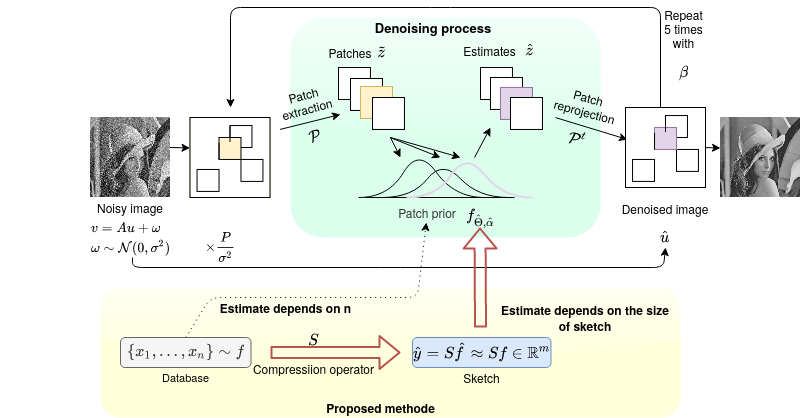
\includegraphics[scale = 0.5]{shema_en.png}
    \caption{Schema of our method}
    \label{fig:shema}
\end{figure}

\textit{Contributions:} The main contributions of this work are the following.
We propose and implement a low-rank model algorithm for the sketching and test the model for image denoising purpose with different parameters.
We further demonstrate the potential of the approach on real large-scale data (over 2 millions training samples) for the task of patch-based image denoising.
We convert some parts of the MATLAB code to python3 in order to make it more accessible.

\textit{Outline:}
The report is organized as follows:
In Section 2, we present the EPLL framework and its usage with GMM priors.
Section 3 is devoted to analyzing the algorithm EM, a classic technique for GMM estimation.
In Section 4, we illustrate the technique of sketching, then we give an implementation with a low-rank technique for GMM estimation in Section 5.
Next, Section 6 provides experimental results both on synthetic data and real images with different parameters.
Finally, we discuss the conclusion and the future perspectives.


\section{Expected Patch Log\hyp{}Likelihood algorithm and its usage under GMM priors}
Image restoration is the operation of estimating the original or underlying clean image from its degraded observations.
Patch-based image restoration algorithms that use priors to do image restoration develop an important category in image restoration.
One of these powerful approaches is the Expected Patch Log\hyp{}Likelihood (EPLL) algorithm introduced by Zoran and Weiss \cite{Zoran}.
It uses priors learned on patches extracted from clean images as a way to regularize corrupted patches.
In this Section, we demonstrate the EPLL framework and its combination with GMM priors.

\subsection{Image restoration with patch-based priors}
We consider the restoration problem by restoring an image $u \in \mathbb{R}^N$ from noisy linear observations $v = \mathcal{A}u+w$, where $\mathcal{A} : \mathbb{R}^N \xrightarrow{} \mathbb{R}^M$ is a linear operator and $w \sim \mathcal{N}(0,\sigma^2 I_M)$ is a white Gaussian noise component.
The EPLL framework which restores an image $u$ by doing a maximum a posteriori (MAP) estimate over all patches correspond to the minimization problem as below:
\begin{equation}\label{eq:op}
    u = \argmin_{u\in \mathbb{R}^N} \frac{P}{2\sigma^2}\|\mathcal{A}u - v \|^2 - \sum_{i = 1}^ N{log(p (\mathcal{P}_i u)})
\end{equation}
where $\mathcal{P}_i : \mathbb{R}^N \xrightarrow{} \mathbb{R}^P$ is the linear operator that extracts a patch with $P$ pixels centered at the position $i$, typically $P = 8 \times 8$ and $p(.)$ is the function of a priori probability distribution.

\subsection{Optimization}
Problem \eqref{eq:op} is a large optimization problem with $p(.)$ often chosen non\hyp{}convex, thus we optimize the problem by using a classic technique: half\hyp{}quadratic splitting.
We introduce N auxiliary unknown vectors $z_i \in \mathbb{R}^P$ and $\beta > 0$, the problem then is considered as:
\begin{equation}\label{eq:2}
    u = \underset{z_1,...,z_N \in R^P}{\argmin_{u\in R^N}} \frac{P}{2\sigma^2}\|\mathcal{A}u - v \|^2 + \frac{\beta}{2}\sum_{i = 1}^N \|\mathcal{P}_i u - z_i\|^2- \sum_{i = 1}^ N{log(p (z_i))}
\end{equation}
When $\beta \xrightarrow{} \infty$, the problem \eqref{eq:2} equals to the original problem \eqref{eq:op}.
The optimization is accomplished by alternating the minimization of $u$ and $z_i$. 
\begin{itemize}
    \item \textbf{Solving u for all fixed $z_i$}\\
    Problem \eqref{eq:2} turns into a linear inverse problem with Tikhonov regularization. It has a solution obtained as:
\begin{equation}
    \hat{u} = \argmin_{u \in \mathbb{R}^N} \frac{P}{2\sigma^2}\|\mathcal{A}u - v \|^2 + \frac{\beta}{2}\sum_{i = 1}^N \|\mathcal{P}_i u - \hat{z_i}\|^2 = \argmin_{u \in \mathbb{R}^N} f(u)
\end{equation}
we have
\begin{equation}
    \nabla f(u) = \frac{P}{\sigma^2}\mathcal{A}^T(\mathcal{A}u-v)+\beta \sum_{i = 1}^N \mathcal{P}_i^T(  \mathcal{P}_i u - \hat{z_i})
\end{equation}
let $\nabla f(u) = 0$, we obtain 
\begin{equation}
    \hat{u} = (\mathcal{A}^T\mathcal{A} + \frac{\beta\sigma^2}{P} \sum_{i = 1}^N \mathcal{P}_i^T \mathcal{P}_i)^{-1}(\mathcal{A}^T v + \frac{\beta\sigma^2}{P} \sum_{i = 1}^N \mathcal{P}_i^T \hat{z_i})
\end{equation}
where $\mathcal{P}_i^T \mathcal{P}_i$ is a diagonal matrix whose $i$\hyp{}th diagonal element corresponds to the number of patches overlapping the pixel in position $i$. 

\item \textbf{Solving $z_i$ for fixed u}\\
Optimizing \eqref{eq:2} leads to :
\begin{equation} \label{eq:3}
    \hat{z_i} = \argmin_{z_1,...,z_N \in \mathbb{R}^P} \frac{\beta}{2}\sum_{i = 1}^N \|\mathcal{P}_i \hat{u} - z_i\|^2- \sum_{i = 1}^ N{log(p (z_i))}
\end{equation}
problem \eqref{eq:3} is a maximum a posteriori denoising problem with the prior of a patch $\mathcal{P}_i \hat{u}$ assumed to be Gaussian with variance $\sigma ^2 = 1/\beta$.
The solution of this problem highly depends on the properties of the chosen patch prior.
\end{itemize}
\subsection{Patch denoising with GMM priors}
In image denoising problem, the linear operator $\mathcal{A}$ in \eqref{eq:op} is identity.
The prior used by EPLL is usually assumed to be a Gaussian mixture model (GMM) prior, for any patch $x \in \mathbb{R}^P$, a GMM is given by 
\begin{equation}\label{eq:gmm}
    p(x) = \sum_{k = 1}^K \alpha_k \mathcal{N}_P(x;\mu_k,\Sigma_k) 
\end{equation}
where $K$ is the number of components, $\alpha_k \in \mathbb{R}^K> 0$ are weights of each component such that $\sum_{k=1}^K \alpha_k = 1$, and $\mathcal{N}_P(x;\mu_k,\Sigma_k)$ denotes the Gaussian distribution with $\mu_k\in \mathbb{R}^P$ and $\Sigma_k \in M_P(\mathbb{R})$ are the corresponding mean and covariance matrix:
\begin{equation}
    \mathcal{N}_P(x;\mu_k,\Sigma_k) = \frac{1}{(2\pi)^{P/2}|\Sigma_k|^{1/2}}\exp (-\frac{1}{2}(x-\mu_k)^T\Sigma_k^{-1}(x-\mu_k))
\end{equation}
Under the GMM prior, problem \eqref{eq:3} leads to:
\begin{equation}
    \hat{z_i} = \argmin_{z_1,...,z_N \in \mathbb{R}^P} \frac{\beta}{2}\sum_{i = 1}^N \|\mathcal{P}_i \hat{u} - z_i\|^2- \sum_{i = 1}^ N{log(\sum_{k = 1}^K \alpha_k \mathcal{N}_P(z_i;\mu_k,\Sigma_k))}
\end{equation}
This problem cannot be solved in closed form as the second term is the logarithm of a sum of exponentials.
Researchers \cite{Zoran} proposed to solve this problem by keeping only the $k_i^*$ component that maximizes the likelihood for the given patch $\tilde{z_i} = \mathcal{P}_i \hat{u}$.
We assume the given patch a Gaussian vector with zero-mean and covariance matrix $\Sigma_{k_i} +\frac{1}{\beta}I_P$. Then $k_i^*$ is chosen by 
\begin{equation}\label{eq:4}
\begin{aligned}
    k_i^* &= \argmax_{1 \leq k_i \leq K} p(k_i|\tilde{z}_i) = \argmax_{1 \leq k_i \leq K}p(k_i)p(\tilde{z}_i|k_i)\\
    & = \argmax_{1 \leq k_i \leq K} \frac{\alpha_{k_i}}{(2\pi)^{P/2}|\Sigma_{k_i}  +\frac{1}{\beta}I_P|^{1/2}}\exp (-\frac{1}{2}(\tilde{z}_i^T(\Sigma_{k_i} +\frac{1}{\beta}I_P)^{-1}\tilde{z}_i)\\
    & = \argmin _{1 \leq k_i \leq K} -2\log\alpha_k + \log \left|\Sigma_{k_i}  +\frac{1}{\beta}I_P\right| + \tilde{z}_i^T(\Sigma_{k_i} +\frac{1}{\beta}I_P)^{-1}z_i
\end{aligned}
\end{equation}
With this assumption, the solution of \eqref{eq:4} is then given by 
\begin{equation}
\begin{aligned}
    \hat{z_i} &= \argmin_{z_1,...,z_N \in \mathbb{R}^P} \frac{\beta}{2}\sum_{i = 1}^N \|\tilde{z_i} - z_i\|^2 + \frac{1}{2}\sum_{i = 1}^ N z_i^T \Sigma_{k_i^*} ^{-1}z_i\\
    &= \argmin_{z_1,...,z_N \in \mathbb{R}^P} f(z_i)
\end{aligned}
\end{equation}
we have 
\begin{equation}
    \nabla f(z_i) = \beta(\tilde{z_i}  - z_i)+\Sigma_{k_i^*} ^{-1}z_i
\end{equation}
let $\nabla f(u) = 0$, we thus obtain 
\begin{equation}\label{eq:5}
    \hat{z_i} = (\Sigma_{k_i^*} +\frac{1}{\beta}I_P)^{-1}\Sigma_{k_i^*}\tilde{z}_i
\end{equation}

\subsection{EPLL framework}
\subsubsection{Algorithm of EPLL}
The EPLL algorithm iterates the 5 steps in Alg. \ref{algo:epll}.
In practice, we perform 5 iterations and follow the settings prescribed in \cite{Zoran}: $\beta = \frac{1}{\sigma^2}\{1,4,8,16,32\}$, the initial $\hat{u}$ is set to $v$.
The author of \cite{Zoran} found that with these parameters, EPLL performances for a large range of noise level.
\begin{algorithm}[htbp]
 \For{\text{all} $i\in I$}{$
 \tilde{z}_i \xleftarrow{} \mathcal{P}_i \hat{u} $\\
$ k_i^* = \argmin _{1 \leq k_i \leq K} -2\log\alpha_k + \log \left|\Sigma_{k_i}  +\frac{1}{\beta}I_P\right| + \tilde{z}_i^T(\Sigma_{k_i} +\frac{1}{\beta}I_P)^{-1}z_i$\\
$ \hat{z_i} = (\Sigma_{k_i^*} +\frac{1}{\beta}I_P)^{-1}\Sigma_{k_i^*}\tilde{z}_i$}
$\tilde{u} = (\sum_{i = 1}^N \mathcal{P}_i^T \mathcal{P}_i))^{-1}\sum_{i = 1}^N \mathcal{P}_i^T \hat{z_i}$\\
$\hat{u} = (A^T A + \beta\sigma^2I_N)^{-1}(A^T v + \beta\sigma^2 \tilde{u})$
 \caption{The 5 steps of EPLL\cite{Zoran}}\label{algo:epll}
\end{algorithm}
\subsubsection{Eigenspace implementation of EPLL}
The matrix inversions in \eqref{eq:4} and \eqref{eq:5} can be done efficiently by storing the eigen decompositions of the covariance matrices.
We denote $\Sigma_k = U_k \Lambda_k U_k^T$, with $U_k \in \mathbb{R}^{P \times P}$ unitary and $\Lambda_k = diag(\lambda_1^k,...,\lambda_P^k)$ where $\lambda_1^k,...,\lambda_P^k$ the eigenvalues of $\Sigma_k$.
Then step 2 and 3 in Alg. \ref{algo:epll} become:
\begin{equation}
    \left\{\tilde{v}_i^k \xleftarrow{} U_k^T \tilde{z}_i \right \}_{\underset{i = 1,...,N}{k = 1,...,K}}
\end{equation}
\begin{equation}
     \left\{k_i^* = \argmin _{1 \leq k \leq K} -2\log\alpha_k + \sum_{j = 1}^P \left( \log (\lambda_j^k + \frac{1}{\beta}) + \frac{[\tilde{v}_i^k]_j^2}{\lambda_j^k + \frac{1}{\beta}}\right)\right \}_{i = 1,...,N}
\end{equation}
\begin{equation}
    \left\{[\hat{v}_i]_j \xleftarrow{} \frac{\lambda_j^{k_i^*}}{\lambda_j^{k_i^*} + \frac{1}{\beta}}[\tilde{v}_i^{k_i^*}]_j\right \}_{\underset{j = 1,...,P}{i = 1,...,N}}
\end{equation}
\begin{equation}
    \left\{ \hat{z}_i \xleftarrow{} U_{k_i^*}\hat{c}_i \right\} _{i = 1,...,N}
\end{equation}
where $[\tilde{v}]_j$ denotes the $j$-th entry of $\tilde{v}$.


\section{Learning GMM priors (Expectation\hyp{}Maximization algorithm)}
The parameters of GMMs can be learned by using the Expectation\hyp{}Maximization (EM) algorithm.
EM is an iterative algorithm to find MAP estimates of parameters, which carries out at each iteration two steps:
 Expectation step (E\hyp{}Step), which creates a function for the expectation of the log\hyp{}likelihood evaluated by using the current estimate for the parameters,
 and Maximization step (M\hyp{}Step), which computes parameters maximizing the expected log\hyp{}likelihood found on the E\hyp{}Step.
These estimated parameters are then used to determine the distribution of the latent variable in the next E\hyp{}Step.
This Section is devoted to analyse EM algorithm.

\subsection{Bayesian's understanding of GMM}
A GMM is given by \eqref{eq:gmm}, we introduce a vector $l= (l_1,...,l_K) \in \mathbb{R}^K$ the latent variable that indicates to which Gaussian component an observation belongs, with $l_k = \{0,1\}$, $\sum_{k =1}^K l_k = 1$, and $p(l_k = 1) = \alpha_k$.
Considering $l_k$ to be independent and identically distributed (i.i.d.), then we have:
\begin{equation}
    p(l) = \prod_{k = 1}^K p(l_k = 1) = \prod_{k = 1}^K \alpha_k^{l_k} 
\end{equation}
\begin{equation}
    p(x|l_k = 1) = \mathcal{N}_P(x;\mu_k,\Sigma_k)
\end{equation}
\begin{equation}
    p(x|l) = \prod_{k = 1}^K p(x|l_k = 1) = \prod_{k = 1}^K \mathcal{N}_P(x;\mu_k,\Sigma_k) ^{l_k}
\end{equation}
According to the Bayes formula:
\begin{equation}
    \begin{aligned}
    p(x) &= \sum_l p(x|l)p(l) \\&= \sum_l \prod_{k = 1}^K 
    \alpha_k^{l_k}\mathcal{N}_P(x;\mu_k,\Sigma_k)^{l_k}
    \\&=\sum_{k = 1}^K \prod_{k = 1}^K \alpha_k^{l_k}\mathcal{N}_P(x;\mu_k,\Sigma_k)^{l_k}
    \\&= \sum_{k = 1}^K \alpha_k\mathcal{N}_P(x;\mu_k,\Sigma_k)
\end{aligned}
\end{equation}
(Note: The third equal in the above formula, summing $l$ is actually $\sum_{k = 1}^K$. Besides, for a given k, if $i \ne k$, $i = 1,...,K$, we have $l_i = 0$, so the term with $l_k = 0$ is 1, which can be ignored in the product.)
    
According to Bayesian method, we can calculate the posterior $p(l|x_i)$ with a prior $p(l_k=1)$ by:
\begin{equation}
    \begin{aligned}
    \Gamma_{i,k}=p(l_k = 1|x_i) &= \frac{p(l_k =1) p(x_i|l_k = 1)}{p(x_i,l_k = 1)}
    \\&= \frac{p(l_k =1) p(x_i|l_k = 1)}{\sum_{j = 1}^K p(l_j=1)p(x_i|l_j = 1)}
    \\& = \frac{\alpha_k \mathcal{N}_P(x_i;\mu_k,\Sigma_k)}{\sum_{j = 1}^K \alpha_j\mathcal{N}_P(x_i;\mu_j,\Sigma_j)}
\end{aligned}
\end{equation}
Above rewrites the form of GMM, and introduces the implicit variable $l$ and the posterior probability $\Gamma_{i,k}$.
This is to facilitate the use of the EM algorithm to estimate the parameters of the GMM.

\subsection{Parameter estimation}
In a GMM, we have three parameters to be estimated: $\Theta_k = (\mu_k, \Sigma_k,\alpha_k)$.
 To estimate these parameters, their the maximum likelihood functions need to be solved separately.
 For training samples $\chi = \{x_1, ...,x_n\}$, the likelihood function of parameter $\Theta_k$ is
\begin{equation}
    \mathcal{L}(\Theta_k; x_1,...,x_n) = \prod_{i = 1}^n  \sum_{k = 1}^K \alpha_k\mathcal{N}_P(x_i;\mu_k,\Sigma_k)
\end{equation}
and the log likelihood is 
\begin{equation}
    log \mathcal{L}(\Theta_k; x_1,...,x_n) = \sum_{i = 1}^n log (\sum_{k = 1}^K \alpha_k\mathcal{N}_P(x_i;\mu_k,\Sigma_k))
\end{equation}
\begin{itemize}
    \item for $\mu_k$, let
\begin{equation}
    \begin{aligned}
    \frac{\partial log  \mathcal{L}(\Theta_k; x_1,...,x_n)}{\partial \mu_k} &= \sum_{i = 1}^n \frac{\partial log (\sum_{k = 1}^K \alpha_k\mathcal{N}_P(x_i;\mu_k,\Sigma_k))}{\partial \mu_k}
    \\&=\sum_{i = 1}^n \frac{\alpha_k\mathcal{N}_P(x_i;\mu_k,\Sigma_k)(x_i - \mu_k)}{\sum_{j = 1}^K \alpha_j\mathcal{N}_P(x_i;\mu_j,\Sigma_j)} C=0
\end{aligned}
\end{equation}    
thus
\begin{equation}\label{eq:mu}
    \mu_k = \frac{1}{N_k}\sum_{i = 1}^n \Gamma_{ik} x_i 
\end{equation}
where $N_k = \sum_{i = 1}^n \Gamma _{i,k} $, $C$ is a constant.
\item for $\Sigma_k$, let
\begin{equation}
    \begin{aligned}
    \frac{\partial log  \mathcal{L}(\Theta_k; x_1,...,x_n)}{\partial \Sigma_k} =& \sum_{i = 1}^n \frac{\partial log (\sum_{k = 1}^K \alpha_k\mathcal{N}_P(x_i;\mu_k,\Sigma_k))}{\partial \Sigma_k}
    \\=&\sum_{i = 1}^n \frac{\alpha_k\mathcal{N}_P(x_i;\mu_k,\Sigma_k)}{\sum_{j = 1}^K \alpha_j\mathcal{N}_P(x_i;\mu_j,\Sigma_j)} \\&[(x_i -\mu_k)^T(x_i -\mu_k)\Sigma_k^{-1} -1] C=0
\end{aligned}
\end{equation}
thus
\begin{equation}\label{eq:sigma}
    \Sigma_k=\frac{1}{N_k}\sum_{i = 1}^n \Gamma _{i,k} (x_i -\mu_k)^T(x_i -\mu_k)
\end{equation}
\item for $\alpha_k$, as it is a constrained optimization problem, we use the method of Lagrange multipliers, which means in order to find the maxima of the function $log \mathcal{L}(\Theta_k; x_1,...,x_n) = log \mathcal{L}(\alpha_k)$ subjected to the equality constraint $\sum_{k=1}^K \alpha _k - 1 = 0$, we find the maxima form the Lagrangian function: 
\begin{equation}
   \mathcal{F}(\alpha_k, \lambda) =  log \mathcal{L}(\alpha_k) + \lambda(\sum_{k=1}^K \alpha _k - 1)
\end{equation}
let $\frac{\partial \mathcal{F}(\alpha_k, \lambda) }{ \partial \alpha_k } = 0$, we get
\begin{equation}
    \frac{\partial \mathcal{F}(\alpha_k, \lambda) }{ \partial \alpha_k } = 
    \sum_{i = 1}^n \frac{\mathcal{N}_P(x_i;\mu_k,\Sigma_k)(x_i - \mu_k)}{\sum_{j = 1}^K \alpha_j\mathcal{N}_P(x_i;\mu_j,\Sigma_j)} + \lambda= 0
\end{equation}
we multiply $\alpha_k$ on each term:
\begin{equation}
     \sum_{i = 1}^n \frac{\mathcal{N}_P(x_i;\mu_k,\Sigma_k)(x_i - \mu_k)}{\sum_{j = 1}^K \alpha_j\mathcal{N}_P(x_i;\mu_j,\Sigma_j)}\alpha_k + \lambda\alpha_k= 0
\end{equation}
so we have
\begin{equation}
    N_k+ \lambda\alpha_k = 0
\end{equation}
\begin{equation}
    \sum_{k=1}^K N_k+ \sum_{k=1}^K \lambda\alpha_k = 0
\end{equation}
\begin{equation}
    \lambda = -\sum_{k=1}^K N_k
\end{equation}{}
thus
\begin{equation}\label{eq:alpha}
    \alpha_k = - \frac{N_k}{\lambda} = \frac{N_k}{\sum_{k=1}^K N_k}
\end{equation}
\end{itemize}

\subsection{EM algorithm}
Parameters estimation using EM algorithm correspond to maximize \eqref{eq:mu}, \eqref{eq:sigma} and \eqref{eq:alpha}.
Given $n$ training clean patches of size $P$, the EM algorithm namely:
\begin{enumerate}
    \item Define the number of component K, for each k, we initialize parameters $\Theta_k = (\mu_k, \Sigma_k,\alpha_k)$, and compute the log likelihood
    \begin{equation}
        log \mathcal{L}(\Theta_k; x_1,...,x_n) = \sum_{i = 1}^n log (\sum_{k = 1}^K \alpha_k\mathcal{N}_P(x_i;\mu_k,\Sigma_k))
    \end{equation}
    \item E\hyp{}Step
    
    Compute $\Gamma_{i,k}$ with the current $\Theta_k$: 
    \begin{equation}
    \Gamma_{i,k} = \frac{\alpha_k \mathcal{N}_P(x_i;\mu_k,\Sigma_k)}{\sum_{j = 1}^K \alpha_j\mathcal{N}_P(x_i;\mu_j,\Sigma_j)}
    \end{equation}
    \item M\hyp{}Step
    
    Update $\Theta_k^{new}$ with the $\Gamma _{i,k}$ obtained in E\hyp{}Step:
    
    \begin{equation}
        \mu_k^{new} = \frac{1}{N_k}\sum_{i = 1}^n \Gamma_{i,k} x_i 
    \end{equation}
    \begin{equation}
        \Sigma_k^{new}=\frac{1}{N_k}\sum_{i = 1}^n \Gamma _{i,k} (x_i -\mu_k)^T(x_i -\mu_k)
    \end{equation}
   \begin{equation}
       \alpha_k^{new} = \frac{N_k}{\sum_{k=1}^K N_k}
   \end{equation}

where $N_k = \sum_{i = 1}^n \Gamma _{i,k} $.
\item Compute the log likelihood of step 1, check if it is converged. 
If not, repeat step 2.
\end{enumerate}
\section{Sketching}
Learning parameters using EM technique face computational issues linked to the size of the data and the number of parameters to estimate, which would make the use of big image databases impractical.
Researchers \cite{keriven:hal-01329195} have proposed a "compressive learning" framework to estimate model parameters from a fixed\hyp{}size representation called \textit{sketch} of the training data.
The dimension of the sketch does not depend on the number of data items in the initial databases.
It would reduce the memory and computational requirements compared to standard techniques.
In this Section, we are going to illustrate the sketching technique. 
\subsection{Compressive mixture estimation}
In the framework of sketching, a distribution $f\in \mathcal{D}$ ($\mathcal{D}$ is the set of probability distributions over $\mathbb{R}^d$) is encoded with a sketching operator $\mathcal{S}: \mathcal{D} \xrightarrow{} \mathbb{C}^m$ into a compressed representation (sketch) $y \in \mathbb{R}^m$:
\begin{equation}
    y = \mathcal{S}f
\end{equation}
the goal is recover $f$. For some finite $K \in \mathbb{N}^*$, we define a K\hyp{}sparse model in $ \mathcal{D} $ with the support $\Theta = \{\theta_1,...,\theta_K\}$ and the weights $\alpha = \{\alpha_1,...,\alpha_K\}$:
\begin{equation}
    f_{\Theta, \alpha} = \sum_{k=1}^K \alpha_k f_{\theta_k}
\end{equation}
where $f_{\theta_k} \in \mathcal{D}$, $\alpha_k \in \mathbb{R}^> 0$ for all components and $\sum_{k=1}^K \alpha_k = 1$. The vector $y$ then can be expressed as 
\begin{equation}
    y = \mathcal{S}f_{\Theta, \alpha} = \sum_{k=1}^K \alpha_k \mathcal{S} f_{\theta_k}
\end{equation}
The algorithm is designed with the purpose of minimizing the measurement error, it corresponds to traditional parametric optimization in the Generalized Method of Moments (GeMM). Given some training data $\chi =\{x_1,...,x_n\} \subset \mathbb{R}^d$, we aim to have:
\begin{equation}\label{eq:sk}
    (\hat{\Theta}, \hat{\alpha}) = \underset{\alpha \in \mathbb{R} ^K, \alpha_k > 0, \sum_{k=1}^K\alpha_k =1}{\argmin_{\Theta \in \mathbb{R} ^K}} \| \hat{y} -\mathcal{S}f_{\Theta, \alpha}\|^2_2
\end{equation}
where $\hat{y} = \mathcal{S}\hat{f}= \frac{1}{n}\sum_{i =1}^n \mathcal{S} \delta_{x_i}$, $ \delta_{x_i}$ is a unit mass at $x_i$.
We want to find the probability mixture whose sketch is closest to the empirical sketch $\hat{y}$.
The sketched learning schema is illustrated in Fig. \ref{fig:sketching}.
The training data are firstly compressed into a smaller representation by applying a sketching operator $S$.
Parameters are then learned from such a compressed representation (sketch) using a learning algorithm adapted to it.
The frequencies $\omega_j$ needed in the construction of the sketching operator can be drawn randomly according to a distribution $\Omega$, possibly designed from a partial preprocessing of the database in practice.
\begin{figure}[h]
    \centering
    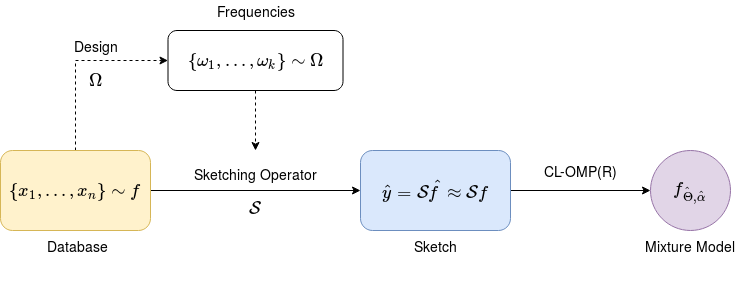
\includegraphics[scale = 0.5]{sketching.png}
    \caption{Paths to compressive learning\cite{keriven:hal-01329195}}
    \label{fig:sketching}
\end{figure}

\subsection{Proposed algorithms: Compressive Learning OMP(R)}
Problem \eqref{eq:sk} is a sparse approximation problem, it can be approximated by greedy algorithms.
One of the algorithms in this category is the Orthonormal Matching Pursuit (OMP) algorithm \cite{article}.
In \cite{keriven:hal-01329195}, two modified algorithms are proposed.
\begin{itemize}
    \item CLOMP (Compressive Learning OMP), which is an adaptation of OMP to the problem
    \item CLOMPR, which is inspired by OMP with Replacement, a variant of OMP that performs more iterations, extends the support further than the desired sparsity and then adds a Hard Thresholding step to reduce the size of support
\end{itemize}
The algorithms are detailed as in Alg. \ref{algo:sk}.

\begin{algorithm}[htbp]
 \KwData{Empirical sketch $\hat{y}$, sketching operator $\mathcal{S}$, sparsity $K$, number of iterations $T \geq K$}
 \KwResult{Support $\Theta$, weights $\alpha$ }
 $\hat{r} \xleftarrow{} \hat{y}$; $\Theta \xleftarrow{} \theta$\;
 \For{t = 1 \textbf{to} $T$ }{
 \textbf{Step 1:} Find a $\theta \in \Theta$ such that:
 $\theta \xleftarrow{} \argmax_\theta Re \left\langle \frac{\mathcal{S}f_\theta}{\|\mathcal{S}f_\theta\|_2}, \hat{r} \right\rangle_2$, init = rand\;
 
 \textbf{Step 2:} $\Theta \xleftarrow{} \Theta \cup \{\theta \}$\;
 
 \textbf{Step 3:} Enforce sparsity by Hard Thresholding if needed\; 
   \If{$|\Theta| > K$}{
   $\eta \xleftarrow{} \argmin_{\eta \geq 0} \left\| \hat{y} - \sum_{k = 1}^{|\Theta|} \eta_k \frac{\mathcal{S}f_{\theta_k}}{\|\mathcal{S}f_{\theta_k}\|_2} \right\|_2^2 $\;
   Select $K$ largest entries $\eta_{i_1},...,\eta_{i_K}$\;
   Reduce the support $\Theta \xleftarrow{} \{ \theta_{i_1},...,\theta_{i_K}\}$\;
 }
 \textbf{Step 4:} Project to find weights\;
 $\alpha \xleftarrow{} \argmin_{\alpha \geq 0} \left\| \hat{y} - \sum_{k = 1}^{|\Theta|} \alpha_k \mathcal{S}f_{\theta_k}\right\| _2^2 $\;
 \textbf{Step 5:} Perform a gradient descent initialized with current parameters\; 
 $\Theta,\alpha \xleftarrow{} \argmin_{\Theta, \alpha \geq 0} \left\| \hat{y} - \sum_{k = 1}^{|\Theta|} \alpha_k \mathcal{S}f_{\theta_k}\right\| _2^2 $, init = ($\Theta,\alpha$)\;
 \textbf{Step 6:} Update residual: 
 $\hat{r} \xleftarrow{} \hat{y} - \sum_{k = 1}^{|\Theta|} \alpha_k \mathcal{S}f_{\theta_k}$;
 }
 Normalize $\alpha$ such that $\sum_{k=1}^K \alpha_k = 1$.

 \caption{Compressive mixture learning: CL\hyp{}OMP ($T = K$) and CL\hyp{}OMPR ($T = 2K$)}
 \label{algo:sk}
\end{algorithm}
Researchers \cite{keriven:hal-01329195} have announced these algorithms can be adapted for any sketching operator $\mathcal{S}$ and any mixture model of parametric densities $f_\theta$ as long as the optimization schemes in Steps 1, 3 and 5 can be performed.

\subsection{Design of sketching operator: randomly sampling the characteristic function}
Researchers \cite{keriven:hal-01329195} propose to draw up the sketch by sampling the characteristic function (\textit{i.e} the Fourier transform) of the probability distribution $f$.
The characteristic function $\psi_f$ of a distribution $f$ is defined as:
\begin{equation}
    \psi_{f}(\omega) = \int_{\mathbb{R}^d} (e^{-i\omega^T x})d f(x) \quad  \forall \omega \in \mathbb{R}^d
\end{equation}
The sketching operator is therefore expressed as:
\begin{equation}
\mathcal{S}f = \frac{1}{\sqrt{m}}[\psi(\omega_1),...,\psi(\omega_m)]^T
\end{equation}
and the sketch is therefore can be calculate by 
\begin{equation}
\begin{aligned}
    y &= \mathcal{S}f_{\Theta, \alpha} = \sum_{k=1}^K \alpha_k \mathcal{S} f_{\theta_k}
\\&=\sum_{k=1}^K \alpha_k \frac{1}{\sqrt{m}}[\psi_{\theta_k}(\omega_1),...,\psi_{\theta_k}(\omega_m)]^T \\&= \frac{K}{\sqrt{m}}\sum_{k=1}^K \alpha_k [\psi_{\theta_k}(\omega_1),...,\psi_{\theta_k}(\omega_m)]^T
\end{aligned}
\end{equation}
Given a training collection $\chi =\{x_1,...,x_n\} \subset \mathbb{R}^d$, we denote the empirical characteristic function $\hat{\psi}(w) = \frac{1}{n} \sum_{i = 1}^n e ^{-i\omega^T x_i}$.
Thus the empirical sketch $\hat{y} = \mathcal{S}\hat{f}$ is:
\begin{equation}
    \hat{y} = \frac{1}{\sqrt{m}}[\hat{\psi}(\omega_1),...,\hat{\psi}(\omega_m)]^T
\end{equation}
One needs to choose the frequencies $\omega_j$, $j = 1...m$ to fully specify the sketching operator.
In the spirit of Random Fourier Sampling, \cite{keriven:hal-01329195} propose to define a probability distribution $\Omega \in \mathcal{D}$ to draw $(\omega_1,...,\omega_m) \sim _{i.i.d.}\Omega$.

\subsection{Sketching Gaussian Mixture Models}
In this Section, we instantiate the proposed framework in the context of GMMs of patches.
Given a training set of $n$ patches $\chi = \{x_1,...,x_n\}$, the density function $f_{\theta_k}$ of each patch $x_i \in \mathbb{R}^P$ is:
\begin{equation}
    f_{\theta_k}(x_i) = \mathcal{N}_P(x_i;\mu_k,\Sigma_k) = \frac{1}{(2\pi)^{P/2}|\Sigma|^{1/2}}\exp(-\frac{1}{2}(x_i-\mu_k)^T\Sigma_k^{-1}(x_i-\mu_k))
\end{equation}
where $\theta_k = (\mu_k,\Sigma_k)$ represents the parameters of the $k$-th Gaussian component with mean $\mu_k \in \mathbb{R}^P$ and covariance $\Sigma_k \in M_P(\mathbb{R})$.
The characteristic function of a Gaussian $f_{\theta_k}$ has a closed\hyp{}form expression as:
\begin{equation}
    \psi_{\theta_k}(\omega) = \exp(-i\omega^T\mu_k)\exp(-\frac{1}{2}\omega^T \Sigma_k \omega) \quad for  \quad \forall \omega \in \mathbb{R}^P
\end{equation}
from which we can derive the expression of the gradients necessary to perform the optimization schemes Steps 1, 3 and 5 in CL\hyp{}OMP(R).

\section{Implementation}
In the work of \cite{keriven:hal-01329195}, a framework to estimate GMMs with diagonal covariances is proposed, which is not sufficient for the task for patch-based image denoising.
Therefore, in this Section, we develop a model to estimate GMMs with non-diagonal covariance.
To reduce the dimension of parameters, we apply a low-rank technique.
Combining the flat-tail spectrum approximation \cite{parameswaran:hal-01617722}, we consider the for the $k$-th Gaussian component, the covariance matrix $\Sigma_k = X_k X_k^T + \rho^2I_P$, where $X_k \in M_{P,r}(\mathbb{R})$ with $r$ the desired rank (see Section \ref{Section:lowrank}) and $\rho^2$ independent from $X_k$. 

\subsection{Code structure}
We implemented a new class, \textbf{gmm\_estimator\_new}, based on the code\footnote{Download from http://sketchml.gforge.inria.fr/} provided by \cite{keriven:hal-01329195}.
Our class uses a low rank technique, and represents the estimator of a GMM with non\hyp{}diagonal covariance.
It inherits from \textbf{mixture\_estimator}, which implements the compressive algorithms for estimating mixtures $f_{\Theta,\alpha} = \sum_{k = 1}^K \alpha_k f_{\theta_k}$ for any model $f_\theta$.
The parameter $\theta = (\mu, X)$ has size $P + P \times r$.

\subsection{Expressions of the necessary gradients}
The core for implementation of Algo. \ref{algo:sk} is to compute the gradients necessary to preform the gradients in Steps 1, 4, and 5. 
\begin{itemize}
    \item \textbf{Step 1:}
    The problem is:
    \begin{equation}
        \theta \xleftarrow{} \argmax_{\theta \in \mathbb{R}^{P+P\times r}} Re \left\langle
    \frac{\mathcal{S}f_\theta}{\|\mathcal{S}f_\theta\|_2}, \hat{r} \right\rangle_2
    \end{equation}
    Denote vector $v(\theta) =[Re(\mathcal{S}f_\theta) ; Im(\mathcal{S}f_\theta)] = [v_1(\theta),...,v_{2m}(\theta)]^T.$
    
    We have for $\forall j = 1,...,m$
    \begin{equation}
    \begin{aligned}
        v_j(\theta) &= Re(\frac{1}{\sqrt{m}}\psi_\theta(\omega_j)) \\
        &= \frac{1}{\sqrt{m}} Re(\exp(-i\omega_j^T\mu_k)\exp(-\frac{1}{2}\omega_j^T \Sigma_k \omega_j))
        \\ &= \frac{1}{\sqrt{m}} \cos{(\omega_j^T\mu_k)}\exp(-\frac{1}{2}\omega_j^T \Sigma_k \omega_j)
        \\ &= \frac{1}{\sqrt{m}} \cos{(\omega_j^T\mu_k)}\exp(-\frac{1}{2}(\omega_j^T X_k X_k^T \omega_j + \sum_{l = 1}^P \omega_{l,j}^2\rho_l^2))
    \end{aligned}
    \end{equation}
    and
    \begin{equation}
        \begin{aligned}
        v_{j+m}(\theta) &= Im(\frac{1}{\sqrt{m}}\psi_\theta(\omega_j)) \\
        &= \frac{1}{\sqrt{m}} Im(\exp(-i\omega_j^T\mu_k)\exp(-\frac{1}{2}\omega_j^T \Sigma_k \omega_j))
        \\ &= -\frac{1}{\sqrt{m}} \sin{(\omega_j^T\mu_k)}\exp(-\frac{1}{2}\omega_j^T \Sigma_k \omega_j)
        \\&= -\frac{1}{\sqrt{m}} \sin{(\omega_j^T\mu_k)}\exp(-\frac{1}{2}(\omega_j^T X_k X_k^T \omega_j + \sum_{l = 1}^P \omega_{l,j}^2\rho_l^2))
    \end{aligned}
    \end{equation}
    Denote $F(\theta) = - Re\left\langle \frac{\mathcal{S}f_\theta}{\|\mathcal{S}f_\theta\|_2}, \hat{r} \right\rangle_2 = - \frac{v(\theta)^T \hat{r}}{\|v(\theta)\|_2}$, where $\hat{r} \in \mathbb{R}^{2m}$, we can compute $\nabla_\theta F(\theta)$ with:
    \begin{equation}
        \begin{aligned}
            \nabla_\theta F(\theta) &= - \frac{1}{\|v(\theta)\|_2^2}((\nabla_\theta v(\theta))^T \hat{r} \|v(\theta)\|_2 -  v(\theta)^T \hat{r} \nabla_\theta \|v(\theta)\|_2) \\&= -\frac{1}{\|v(\theta)\|_2^2}((\nabla_\theta v(\theta))^T \hat{r} \|v(\theta)\|_2 -  \frac{v(\theta)^T \hat{r}(\nabla_\theta v(\theta) )^T v(\theta) }{\|v(\theta)\|_2} )
        \\&= - \frac{(\nabla_\theta v(\theta) )^T }{\|v(\theta)\|_2} (\hat{r}-\frac{v(\theta)^T \hat{r} v(\theta)}{\|v(\theta)\|_2^2})  
        \\&=  - \frac{(\nabla_\theta v(\theta) )^T }{\|v(\theta)\|_2} (\hat{r}-\frac{F(\theta)v(\theta)}{\|v(\theta)\|_2})  
                \\&=  \frac{(\nabla_\theta v(\theta) )^T }{\|v(\theta)\|_2} (\frac{F(\theta)v(\theta)}{\|v(\theta)\|_2} -\hat{r}) 
        \end{aligned}
    \end{equation}
Then we need to calculate $\nabla_{\theta} v(\theta)$, i.e. %$\nabla_{X_k} v(X_k)$. 
$\nabla_{\theta} v(\theta)  = [\nabla_{\mu_k} v(\mu_k);\nabla_{X_k} v(X_k)]$. 
\begin{itemize}
   \item Compute $\nabla_{\mu_k} v(\mu_k)$\\
   For $\forall j = 1,...,m$:
\begin{equation}
    \begin{aligned}
    \nabla_{\mu_k} v_j(\mu_k) &= \frac{1}{\sqrt{m}} (-\sin{(\omega_j^T\mu_k)}\omega_j)\exp(-\frac{1}{2}\omega_j^T \Sigma_k \omega_j)
        \\&= -\frac{1}{\sqrt{m}} \sin{(\omega_j^T\mu_k)}\omega_j\exp(-\frac{1}{2}\omega_j^T \Sigma_k \omega_j) 
        \\&= v_{j+m}(\theta) \omega_j
    \end{aligned}
\end{equation}
and 
\begin{equation}
\begin{aligned}
        \nabla_{\mu_k} v_{j+m}(\mu_k) &= -\frac{1}{\sqrt{m}} \cos{(\omega_j^T\mu_k)}\omega_j\exp(-\frac{1}{2}\omega_j^T \Sigma_k \omega_j)
    \\&=-v_j(\theta)\omega_j 
\end{aligned}
\end{equation}
In practice, given $W = [\omega_1,...,\omega_m]$ the frequencies matrix, with $\omega_j \in \mathbb{R}^P, j = \{1,...,m\} $, $y \in \mathbb{R}^{2m}$, according to (5.5), (5.6), we have
\begin{equation}
    \begin{aligned}
        (\nabla_{\mu_k} v(\mu_k) )^T y &= \langle \nabla_{\mu_k} v(\mu_k) , y \rangle \\&=
        v(\theta)_{m+1:2m} \dot* y_{1:m} * w_{1:m} - v(\theta)_{1:m} \dot* y_{m+1:2m} * w_{1:m}
        \\&= W*(v(\theta)_{m+1:2m} \dot* y_{1:m} - v(\theta)_{1:m} \dot* y_{m+1:2m})
    \end{aligned}
\end{equation}
where $\dot*$ denote the multiplication element by element.
\item Compute $\nabla_{X_k} v(X_k)$ \\
We have
\begin{equation}
    \nabla_{X_k} v_j(X_k) = - \frac{1}{2\sqrt{m}}  \exp(-i\omega_j^T\mu_k)  \exp(-\frac{1}{2}\omega_j^T \Sigma_k \omega_j)\nabla_{X_k} g_j(X_k)
\end{equation}
with $g_j(X_k)$ calculated as
\begin{equation}
    \begin{aligned}
    g_j(X_k) &= \omega_j^T \Sigma_k \omega_j = \omega_j^T (X_k X_k^T + \rho^2 I_P)\omega_j \\&= \omega_j^T X_k X_k^T \omega_j + \omega_j ^T \rho^2 \omega_j
    \\&= (X_k^T \omega_j)^T(X_k^T \omega_j)+ \omega_j ^T \rho^2 \omega_j \\& = \langle X_k^T \omega_j, X_k^T \omega_j \rangle + \omega_j ^T \rho^2 \omega_j
\end{aligned}
\end{equation}
thus the derivative of $g_j(X_k)$ on element $x_{l,s}$ is:
\begin{equation}
    \begin{aligned}
    \frac{\partial g_j(X_k)}{\partial x_{l,s}^k} &= 2 \langle \frac{\partial X_k^T \omega_j}{\partial x_{l,s}^k}   ,X_k^T \omega_j \rangle \\&= 2 \langle E_{l,s}^k \omega_j ,X_k^T \omega_j \rangle \\&= 2\omega_j ^T (E_{l,s}^k)^T X_k^T \omega_j\\&= 2\omega_j ^T (X_k E_{l,s}^k)^T \omega_j
\end{aligned}
\end{equation}
with $E_{l,s}^k \in M_{r, P}(\mathbb{R}) $ and its element $e_{i,j}^k = \begin{cases} 1 & \mbox{if } \{i, j\} = \{s, l\} \\ 0 & \mbox{other wise}  \end{cases}$. 

So we have 
\begin{equation}
    \frac{\partial v_j(X_k)}{\partial x_{l,s}^k} = - \frac{1}{\sqrt{m}}  \exp(-i\omega_j^T\mu_k)  \exp(-\frac{1}{2}\omega_j^T \Sigma_k \omega_j)\omega_j ^T (X_k E_{l,s}^k)^T  \omega_j
\end{equation}
For $\forall j = 1,...,m$:
\begin{equation}
\begin{aligned}
        \frac{\partial v_j(X_k)}{\partial x_{l,s}^k} &= - \frac{1}{\sqrt{m}}  \cos(\omega_j^T\mu_k)  \exp(-\frac{1}{2}\omega_j^T \Sigma_k \omega_j)\omega_j ^T (X_k E_{l,s}^k)^T  \omega_j
        \\&= - v_j(\theta)\omega_j ^T (X_k E_{l,s}^k)^T  \omega_j
\end{aligned}
\end{equation}

\begin{equation}
\begin{aligned}
    \frac{\partial v_{j+m}(X_k)}{\partial x_{l,s}^k} &=  \frac{1}{\sqrt{m}}  \sin(\omega_j^T\mu_k)  \exp(-\frac{1}{2}\omega_j^T \Sigma_k \omega_j)\omega_j ^T (X_k E_{l,s}^k)^T  \omega_j \\&= - v_{j+m}(\theta)\omega_j ^T (X_k E_{l,s}^k)^T  \omega_j
    \end{aligned}
\end{equation}
Denote $\mathcal{Y}_{l,s}^k = (X_k E_{l,s}^k)^T$, according to calculation, we can express $\mathcal{Y}_{l,s}^k$ as
\begin{equation}
    \mathcal{Y}_{l,s}^k(l,:) = \begin{cases} X_k(:,s) & \mbox{with}\quad 1 \leq l \leq P, 1 \leq s \leq r\\ 0 & \mbox{other wise}  \end{cases}
\end{equation}
In practice, given $W = [\omega_1,...,\omega_m]$, with $\omega_j \in \mathbb{R}^P, j = \{1,...,m\} $ the frequencies matrix, $y \in \mathbb{R}^{2m}$, we have
\begin{equation}
    \begin{aligned}
        (\nabla_{X_k} v(X_k) )^T y &= \langle \nabla_{X_k} v(X_k) , y \rangle 
        \\&= -W_2(v(\theta)_{1:m} \dot* y_{1:m} + v(\theta)_{m+1:2m} \dot* y_{m+1:2m})
    \end{aligned}
\end{equation}
where $W_2 \in M_{J , m}(\mathbb{R})$ with $J = P\times r$ and its $j$th $(1 \leq j \leq J)$ component can be expressed as:
\begin{equation}
    W_2(j,:) = \mathcal{Y}_{l,s}^k(:,s)^T  W \dot * W(s,:) = X_k(:,l)^T  W \dot * W(s,:)
\end{equation}
with $ j= (l-1)d+s$ and $\dot*$ the multiplication element by element.
\end{itemize}
\item \textbf{Step 3:}
    The problem is 
    \begin{equation}
        \eta \xleftarrow{} \argmin_{\eta \geq 0} \left\| \hat{y} - \sum_{k = 1}^{|\Theta|} \eta_k \frac{\mathcal{S}f_{\theta_k}}{\|\mathcal{S}f_{\theta_k}\|_2} \right\|_2^2 
    \end{equation}
    Denote $V = [\frac{v(\theta_1)}{\|v(\theta_1)\|_2} ,  ...,\frac{v(\theta_K)}{\|v(\theta_K)\|_2}]$, $\eta = [\eta_1,...,\eta_K]^T$, then we have
    \begin{equation}
        \begin{aligned}
        g(\eta)&= \left\| \hat{y} - \sum_{k = 1}^{|\Theta|} \eta_k \frac{\mathcal{S}f_{\theta_k}}{\|\mathcal{S}f_{\theta_k}\|_2} \right\|_2^2  \\&= \left\| \hat{y} - \sum_{k = 1}^{|\Theta|} \eta_k \frac{v(\theta_k)}{\|v(\theta_k)\|_2} \right\|_2^2
        \\&= \| \hat{y} - V\eta  \|_2^2
    \end{aligned} 
    \end{equation}
    we have 
    \begin{equation}
        \begin{aligned}
        \nabla _\eta g(\eta) &= 2\langle  \hat{y} - V\eta  , -V \rangle \\ &= 2\langle V, V\eta  - \hat{y}  \rangle \\&= 2 V^T (V\eta  - \hat{y} )
        \end{aligned}
    \end{equation}
    \item \textbf{Step 5:}
    The problem is 
    \begin{equation}
        (\Theta,\alpha) \xleftarrow{} \underset{\alpha \in \mathbb{R} ^K, \alpha_k > 0, \sum_{k=1}^K\alpha_k =1}{\argmin_{\Theta \in  \mathbb{R} ^K, \theta_k \in \mathbb{R}^{P+P\times r}}} \left\| \hat{y} - \sum_{k = 1}^{|\Theta|} \alpha_k \mathcal{S}f_{\theta_k}\right\| _2^2 
    \end{equation}
    Denote $V = [v(\theta_1),  ...,v(\theta_K)]$, $\alpha = [\alpha_1,...\alpha_K]^T$, then 
    \begin{equation}
        \begin{aligned}
        h(\Theta,\alpha)&= \left\| \hat{y} - \sum_{k = 1}^{|\Theta|} \alpha_k \mathcal{S}f_{\theta_k}\right\| _2^2 \\&= \left\| \hat{y} - \sum_{k = 1}^{|\Theta|} \alpha_k v(\theta_k)\right\| _2^2
        \\&= \| \hat{y} - V\alpha  \|_2^2
    \end{aligned} 
    \end{equation}
    we have 
    \begin{equation}
        \nabla _\alpha h(\Theta,\alpha) = 2 V^T (V\alpha  - \hat{y} )
    \end{equation}
    and 
    \begin{equation}
        \begin{aligned}
            \nabla _{\theta_k} h(\Theta,\alpha)&= 2\langle \hat{y} - V\alpha , -\nabla_{\theta_k} V\alpha \rangle \\&=  2\langle \hat{y} - V\alpha , - \alpha_k \nabla_{\theta_k} v(\theta_k) \rangle \\&= 2\alpha_k \nabla_{\theta_k} v(\theta_k)^T (V\alpha - \hat{y})
        \end{aligned}
    \end{equation}
\end{itemize}

\subsection{Flat-tail spectrum approximation}\label{Section:lowrank}
As Gaussian models on patches are usually over-parameterized, we use a simple and standard eigenvalue-based regularization: $\Sigma_k \xleftarrow{} A_k + \rho^2 I_P$, where $\rho^2$ is a small constant independent.
We rely on a flat-tail approximation: pose low rank constraints to make the model easy to infer and reduce the overall computational complexity.
Since the matrix $\Sigma_k$ is symmetric positive semi-definite, denote $A_k = \Sigma_k - \rho^2 I_P \in M_P(\mathbb{R})$ is a real symmetric and positive definite matrix and it can be expressed as $A_k = U_k \Lambda_k U_k^T$, where $U_k$ is a full-rank orthogonal matrix whose columns are the eigenvectors of $A_k$, and $\Lambda_k$ is a diagonal matrix containing the positive eigenvalues of $A_k$.
We can define $\Lambda_k^{1/2} \in M_P(\mathbb{R})$ to be the diagonal matrix whose diagonal elements are the square roots of the corresponding diagonal elements of $\Lambda_k$.
We have consequently
\begin{equation}
    A_k= U_k \Lambda_k U_k^T = U_k \Lambda_k^{1/2} (\Lambda_k^{1/2})^T U_k^T = U_k \Lambda_k^{1/2} (U_k \Lambda_k^{1/2})^T = X_k X_k^T 
\end{equation}
$\Sigma_k$ is flat-tail if there exist a rank $r$ as for any $j > r$ the eigenvalues of $\Sigma_k$ are constant. In practice, the Gaussian covariance $\Sigma_k$ is not flat-tail but can be approximated by a 
Given the rank $r$, we can approximate $X_k$ with $X_k = U_k \Lambda_{k,r}^{1/2}$, where $\Lambda_{k,r}^{1/2}$ is the submatrix of $\Lambda_k^{1/2}$ formed with the first $r$ columns of $\Lambda_k^{1/2}$.


\section{Results and analysis}
In this Section, we give several numerical experiments to show the model's characteristics and its denoising performance.
We show experimental results on synthetic data in Section \ref{Section:syn data}, then we provide results on image denoising with models learned by sketching and compare them with models estimated by EM algorithm in Section \ref{Section:res img}. 

\subsection{Evaluation measure}
To evaluate the reconstruction performance of model $f_{\Theta, \alpha}$, we observe the model's energy expressed as
\begin{equation}
    E(\hat{y}, f) = \left \|\hat{y} - Sf\right\|_2^2
\end{equation}
with $\hat{y}$ the empirical sketch and $S$ the sketch operator.
We use PSNR (Peak signal to noise ratio) and SSIM (Structural similarity) to measure the reconstruction quality of a restored image $\hat{u}$ compared to its degraded one $u$. 
For an image with pixel values between 0 and 1, the PSNR is computed by 
\begin{equation}
    \text{PSNR}(\hat{u},u) = 10 \log_{10}\frac{N}{\sum_{i=1} ^N(\hat{u}(i) - u(i))^2}
\end{equation}
where $N$ is the number of pixel in image $u$. The SSIM between two patches $x \in u$ and $y \in \hat{u}$ is given by the formula
\begin{equation}
    \text{SSIM}(x,y) = \frac{(2\mu_x\mu_y + c_1)(2\sigma_{xy} + c_2)}{(\mu_x^2 + \mu_y^2 + c_1)(\sigma_x^2 + \sigma_y^2 + c_2)}
\end{equation}
where $\mu_x, \sigma_x^2$ (resp.$\mu_y, \sigma_y^2$) are the mean and variance of $x$ (resp.$y$), $\sigma_{xy}$ the covariance of $x$ and $y$, $c_1$ and $c_2$ are two variables to stabilize the division with weak denominator. 

\subsection{Experiments with synthetic data}\label{Section:syn data}
\subsubsection{Results: low dimension estimation}
We first test our model on 2 type of data (GMMs with zero-means, diagonal covariances and non-diagonal covariances) generated in 2-dimensions ($d = 2$).
For each test we draw $n = 100000$ items with the settings: the sparsity level of GMM $K = 2$, the frequencies of sketch $m = 500$, the desired rank $r=1$.
Reconstruction is performed with the algorithm CL\hyp{}OMPR. Fig. \ref{fig:syn} shows the model estimation results. 
\begin{figure}[h]
    \begin{minipage}[t]{.45\textwidth}
      \centerline{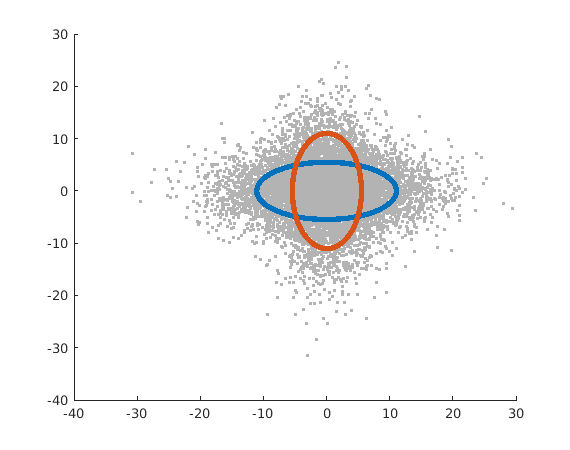
\includegraphics[scale=0.5]{t1.png}}
    \end{minipage}
    \begin{minipage}[t]{.45\textwidth}
      \centerline{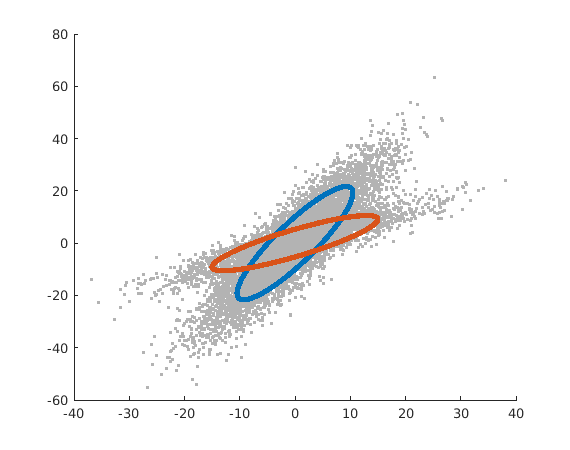
\includegraphics[scale=0.5]{t2.png}}
    \end{minipage}
    \caption{Modeling on synthetic data}
    \label{fig:syn}
\end{figure}
\subsubsection{Results: comparison with EM algorithm}
We also compared the reconstruction performance with EM algorithm implemented in Matlab\footnote{MATLAB code downloaded from http://www.mathworks.com/matlabcentral/fileexchange \allowbreak /26184-em-algorithm-for-gaussian-mixture-model} by using the same generated data with the settings: we draw $n = 100000$ items, dimension $d = 4$, the sparsity level of GMM $K = 8$.
For the sketching, the frequencies $m = 500$, the rank $r$ is set to 2.  Fig. \ref{fig:2} shows the reconstruction performance (projected on the first 2 dimensions).
On synthetic data, the sketching method produces precis results while needing less iterations to converge, we do experiences for 50 times with the same settings and obtain the mean calculate time as shown in the table.
\begin{figure}[h]
    \begin{minipage}[t]{.45\textwidth}
      \centerline{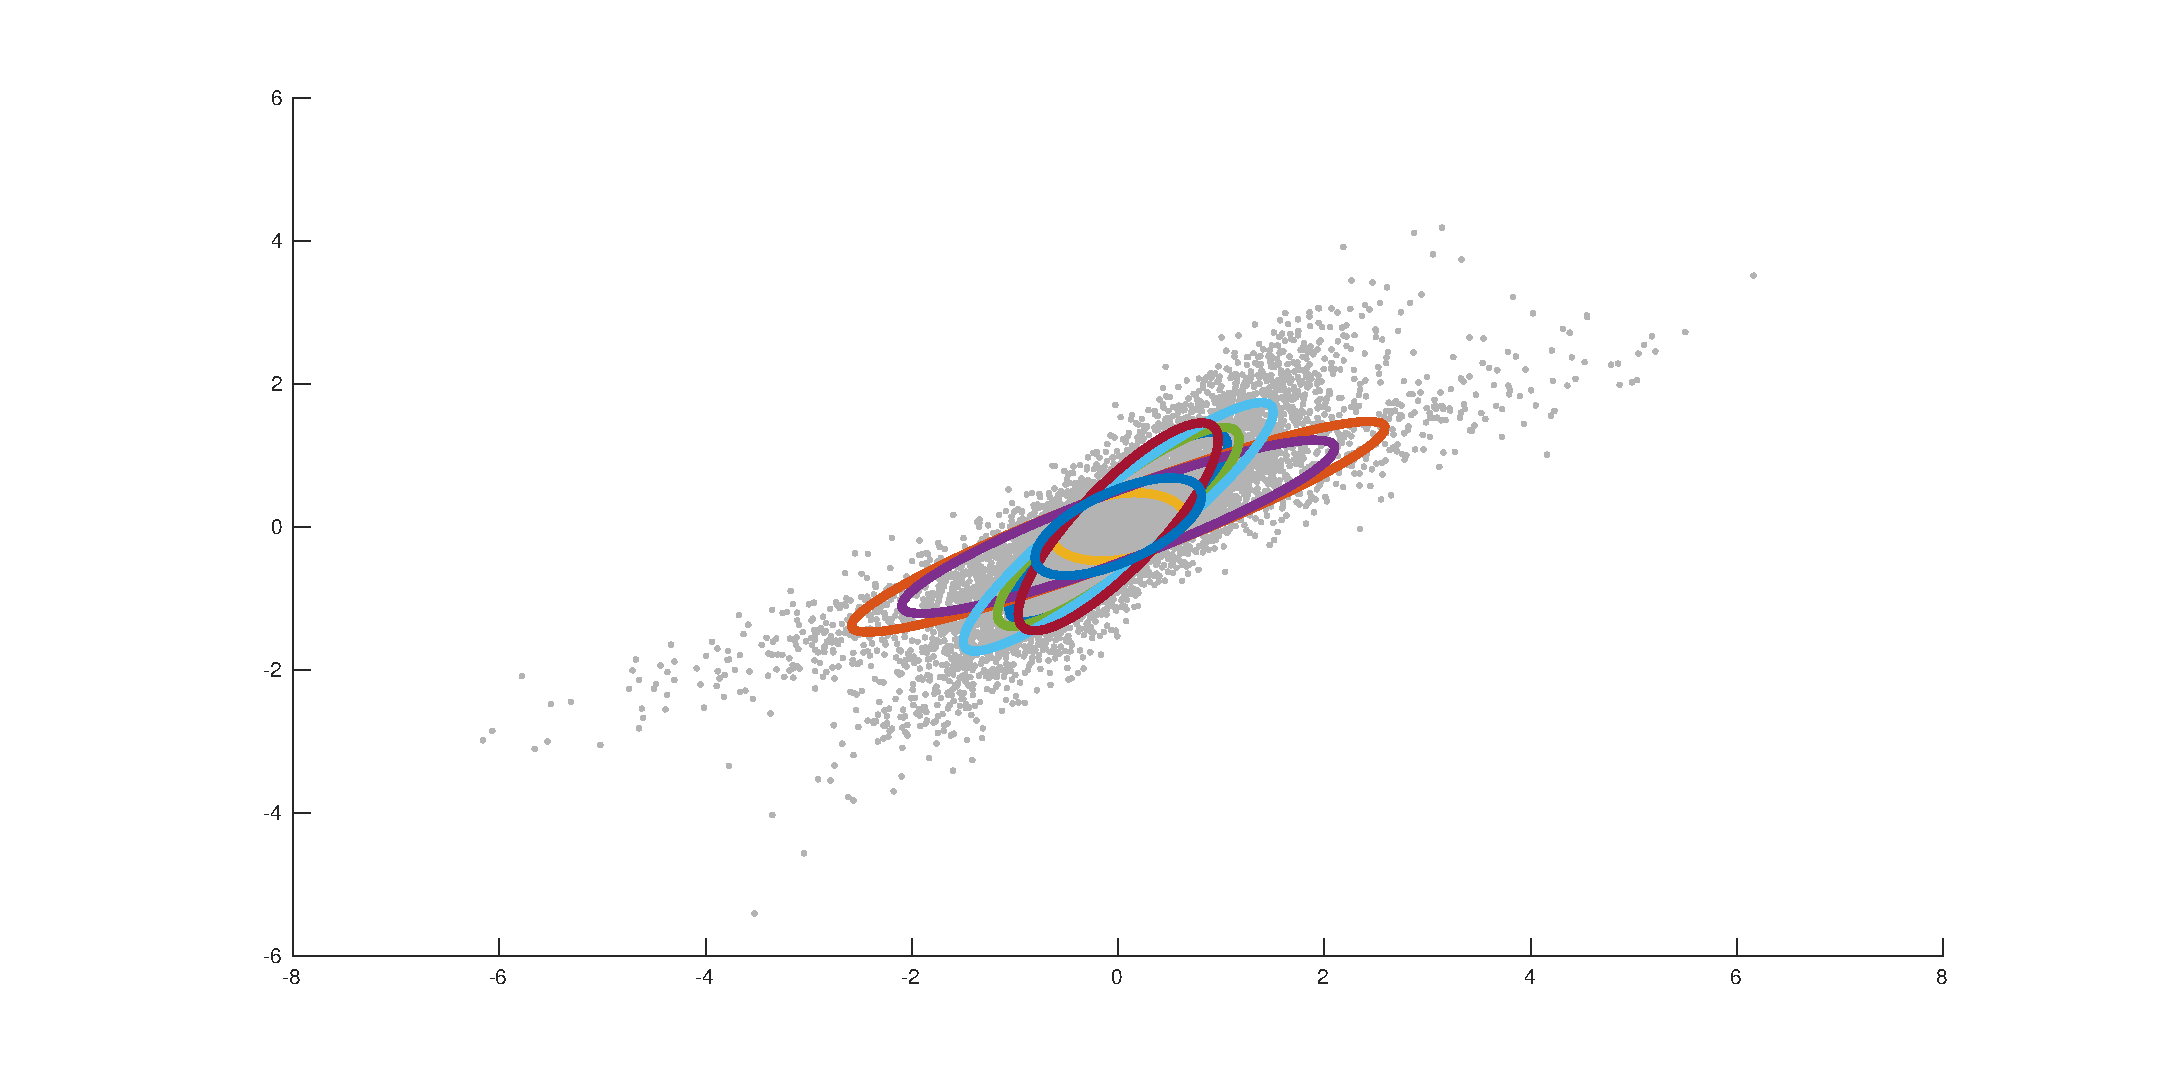
\includegraphics[scale=0.25]{data_sk.eps}}
    \end{minipage}
    \begin{minipage}[t]{.45\textwidth}
      \centerline{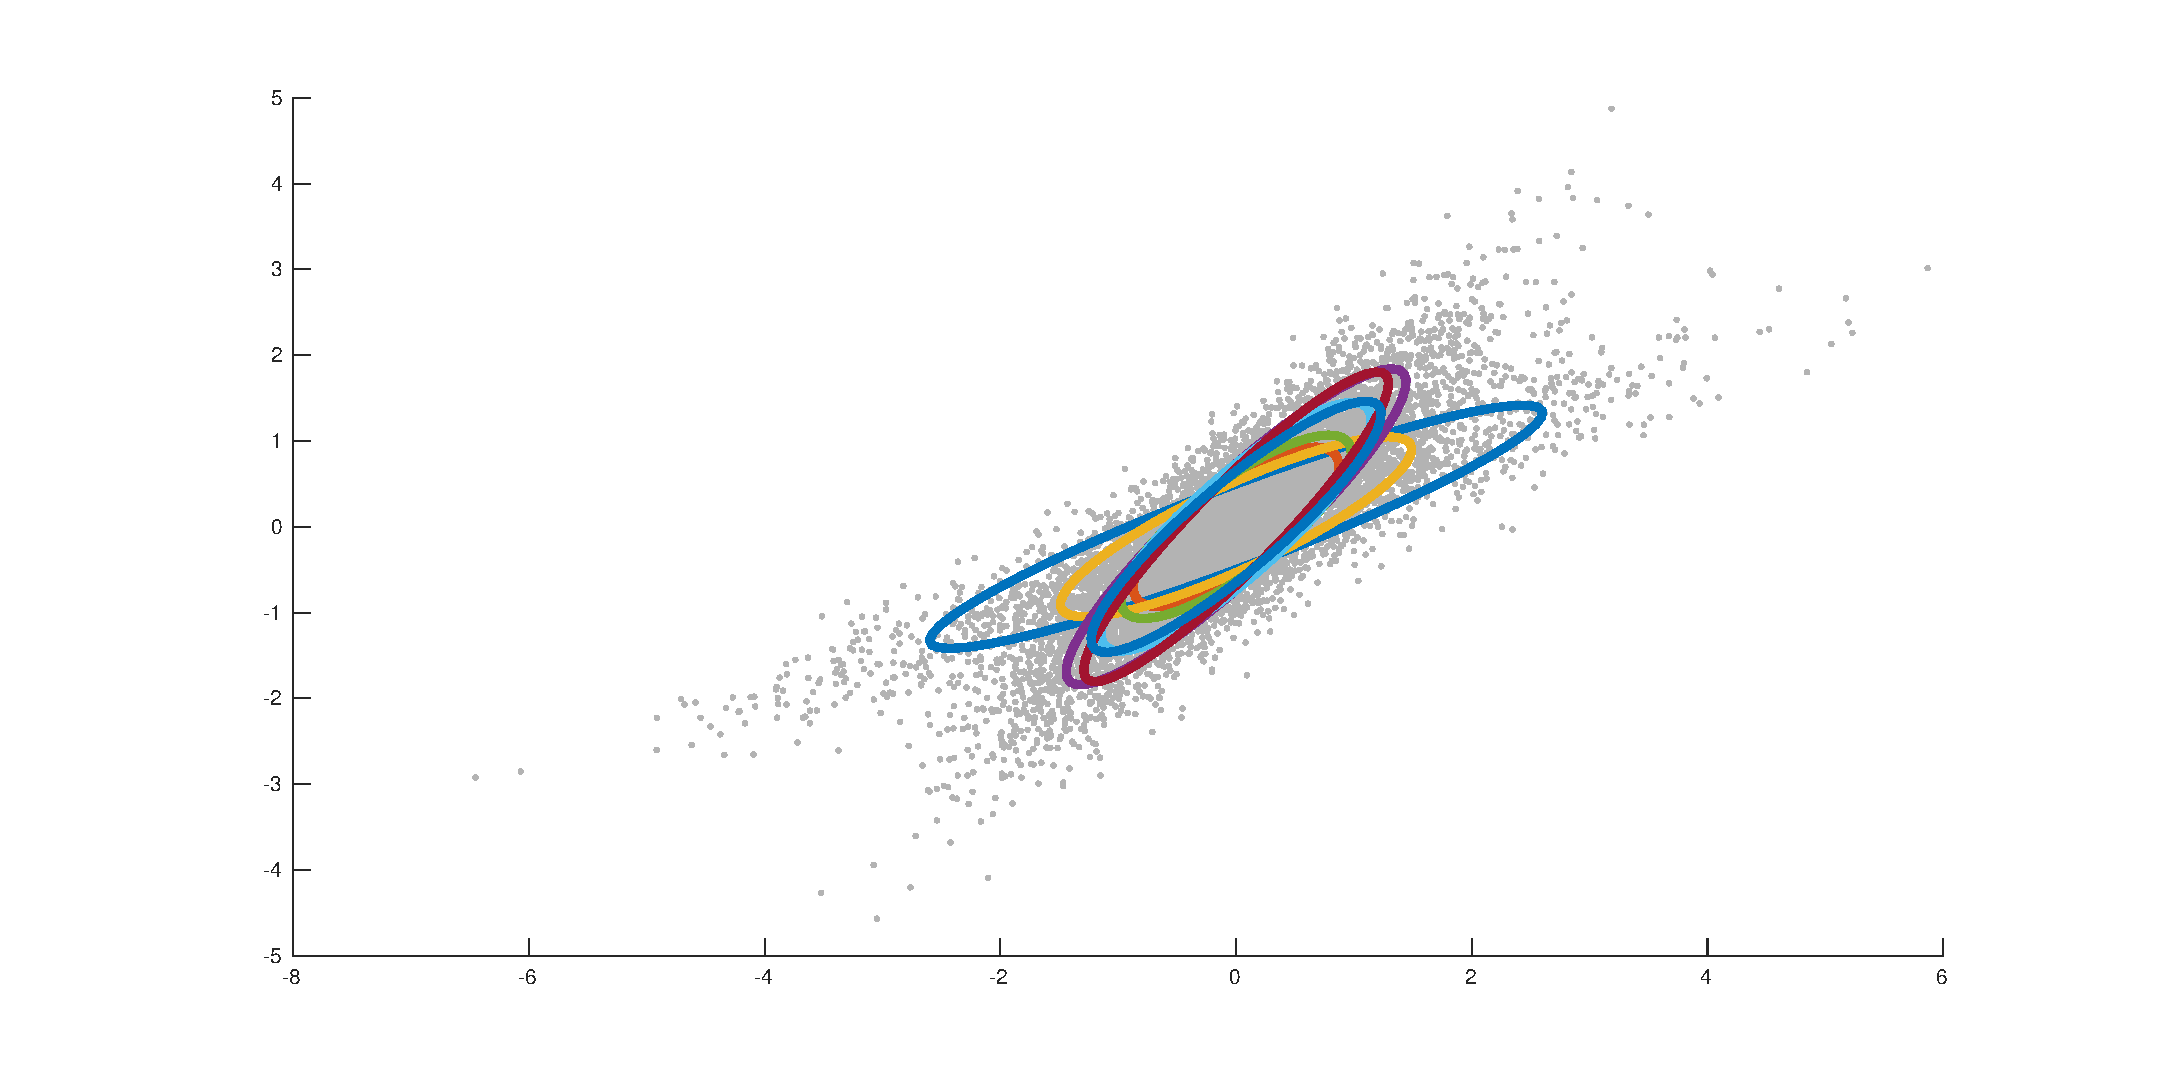
\includegraphics[scale=0.25]{data_em.eps}}
    \end{minipage}
    \caption{Modeling on synthetic data with sketching(left) and EM(right)}
    \label{fig:2}
\end{figure}
\begin{table}[h]\centering
\begin{tabular}{|c|c|c|}
\hline
 & \bfseries Sketching & \bfseries EM \\
\hline
\bfseries Time  & 2.0091s & 11.877s \\
\hline
\end{tabular}
\caption{The average calculate time using the 2 methods on synthetic data}
\end{table}

\subsection{Results on the real image}\label{Section:res img}
For the following Sections, tests are done on noisy images (\textit{cameraman} and \textit{barbara}) generated by adding a Gaussian noise $\omega \sim \mathcal{N}(0, 20)$ on the original ones (Fig. \ref{fig:or and noisy}).
In this Section, we illustrate the denoising performance of models with different parameters: $r$ and $\rho^2$ for low-rank approximation of $\Sigma_k$, the sparsity level $K$, the size of sketch $m$ and the number of iterations during the learning process.
We extract randomly $2 \times 10^5$ patches of size $P = 8 \times 8$ from the training images of Berkeley Segmentation Database (BSDS)\footnote{https://www2.eecs.berkeley.edu/Research/Projects/CS/vision/bsds/} for the experiments.
\begin{figure}[h]
    \centering
    \begin{tabular}{cc}
    cameraman & barbara \\
    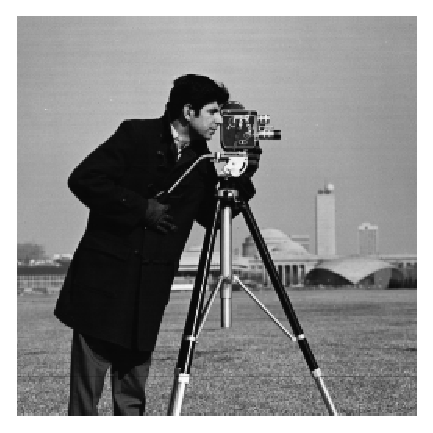
\includegraphics{or_ca.eps} & 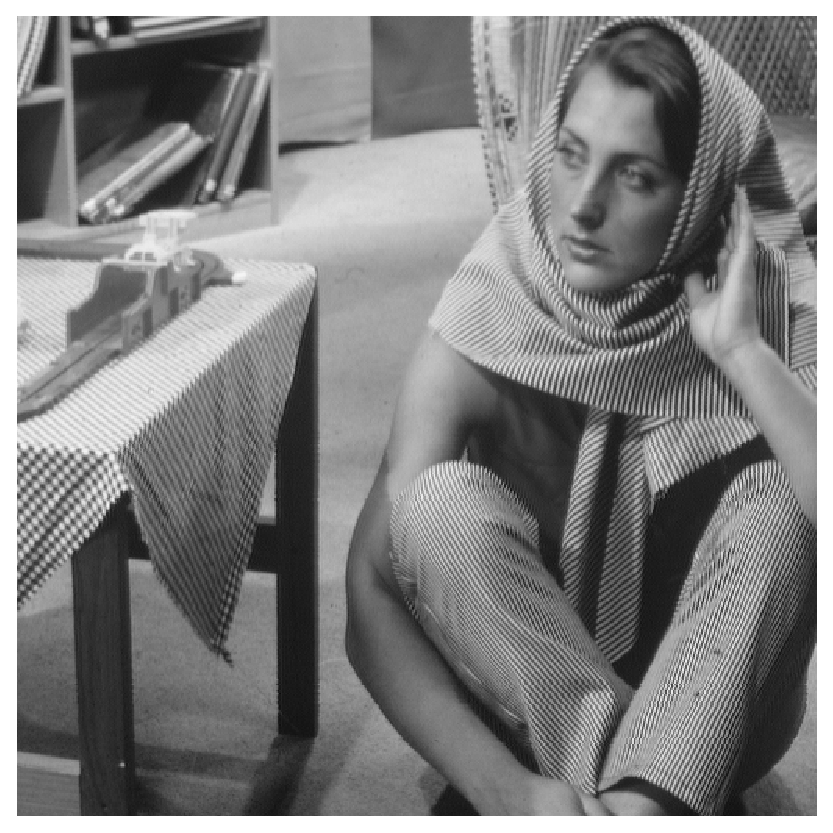
\includegraphics[scale=0.5]{or_bar.eps} \\
    \includegraphics<\put (0,0){\fcolorbox{white}{white}{\textcolor{black}{22.1/.403}}}>{noisy_ca.eps} & \includegraphics[scale=0.5]<\put (0,0){\fcolorbox{white}{white}{\textcolor{black}{22.1/.479}}}>{noisy_bar.eps}
   \end{tabular}
   \caption{Original and noisy images for tests with PSNR/SSIM}
   \label{fig:or and noisy}
\end{figure}
\subsubsection{Experiments on $r$}
To avoid computing all the coefficients, we apply the flat-tail approximation for the covariance matrix.
In this Section, we test different ranks $r$ to see their influence in denoising performance, \cite{parameswaran:hal-01617722} mentions in practice an average of $r = 19.6$ leads to a small drop of PSNR (0.1dB).
From top to bottom, Fig. \ref{fig:diff r} shows the denoised results on \textit{cameraman} and \textit{barbara} by EPLL\footnote{MATLAB code download from https://goo.gl/xjqKUA} using models estimated by sketching with $r$ = 5, 10 and 19, the other parameters are fixed with $\rho^2 = 1e-4, K = 20, m = 5K(P+P\times r+1)$, we can see a coherent result that while $r$ increase PSNR and SSIM values also augment.
For the future tests, we simply set $r = 19$ for a good and fast results.
\begin{figure}[h]
    \centering
    \begin{tabular}{ccc}
\rotatebox{90}{$r=5$} & \includegraphics<\put (0,0){\fcolorbox{white}{white}{\textcolor{black}{22.6/.714}}}>{r5cam.eps} & \includegraphics[scale=0.5]<\put (0,0){\fcolorbox{white}{white}{\textcolor{black}{23.7/.669}}}>{r5bar.eps} \\
\rotatebox{90}{$r=10$} & \includegraphics<\put (0,0){\fcolorbox{white}{white}{\textcolor{black}{24.9/.786}}}>{r10cam.eps} & \includegraphics[scale=0.5]<\put (0,0){\fcolorbox{white}{white}{\textcolor{black}{24.6/.721}}}>{r10bar.eps} \\
\rotatebox{90}{$r=19$} & \includegraphics<\put (0,0){\fcolorbox{white}{white}{\textcolor{black}{26.4/.814}}}>{r19cam.eps} & \includegraphics[scale=0.5]<\put (0,0){\fcolorbox{white}{white}{\textcolor{black}{25.4/.753}}}>{r19bar.eps}
    \end{tabular}
    \caption{Denoised results using different $r$ with PSNR/SSIM}
    \label{fig:diff r}
\end{figure}
\subsubsection{Experiments on $\rho^2$}
Our tests in this Section was to find the optimal parameter $\rho$, we fix other parameters as $K= 20$, the frequencies of sketch $m = 5K(P+P\times r +1)$ and the rank $r=19$.
Denote the patch covariance matrix of the $k$-th group $\Sigma_k = U_k\Lambda_k U_k^T + \rho^2$, we test $\rho^2$ with different values to find the optimal one for denoising purpose.
Fig. \ref{fig:diff rho} shows the denoised results on \textit{cameraman} and \textit{barbara} with different $\rho^2$: $1e-4$ for images in the first row, $1e-5$ for images in the second row and $1e-6$ in the third row.
We can see from the figure that when $\rho^2 = 1e-4$ we obtain a better denoising performance.
\begin{figure}[h]
    \centering
    \begin{tabular}{ccc}
    \rotatebox{90}{$\rho^2=1e-4$} & \includegraphics<\put (0,0){\fcolorbox{white}{white}{\textcolor{black}{26.4/.814}}}>{rho_1e-4.eps} & \includegraphics[scale=0.5]<\put (0,0){\fcolorbox{white}{white}{\textcolor{black}{25.4/.753}}}>{rho_bar_1e-4.eps}\\
    \rotatebox{90}{$\rho^2=1e-5$} & \includegraphics<\put (0,0){\fcolorbox{white}{white}{\textcolor{black}{26.3/.817}}}>{k_20.eps} & \includegraphics[scale=0.5]<\put (0,0){\fcolorbox{white}{white}{\textcolor{black}{25.3/.753}}}>{k_20_bar.eps} \\
    \rotatebox{90}{$\rho^2=1e-6$} & \includegraphics<\put (0,0){\fcolorbox{white}{white}{\textcolor{black}{25.7/.804}}}>{rho_1e-6.eps} & \includegraphics[scale=0.5]<\put (0,0){\fcolorbox{white}{white}{\textcolor{black}{24.9/.734}}}>{rho_bar_1e-6.eps}
    \end{tabular}
    \caption{Denoised results using different $\rho^2$ with PSNR/SSIM}
    \label{fig:diff rho}
\end{figure}
\textbf{Search for the optimal $\beta$}\\
The denoised images in Fig. \ref{fig:diff r} and Fig. \ref{fig:diff rho} are obtained by applying EPLL for 5 iterations with $\beta = \frac{1}{\rho^2}\{1,4,8,16,32\}$ in equation \eqref{eq:op} as in \cite{parameswaran:hal-01617722} and \cite{deledalle:hal-01700082}.
In order to have a better denoising performance, we modify the value of $\beta$. We did 2 tests on \textit{cameraman} to find out the optimal $\beta$:
\begin{enumerate}
    \item We run EPLL for 5 iterations while with successive values $\beta' = n\beta$ instead, $n$ varies between 0.01 and 5. Fig. \ref{fig:test1} illustrate the variations of PSNR and SSIM with $n$, we zoom in the segment [0.01, 1] and illustrate it in Fig. \ref{fig:test1 zoom in}. 
    \begin{figure}[h]
        \begin{minipage}[t]{.5\textwidth}
          \centerline{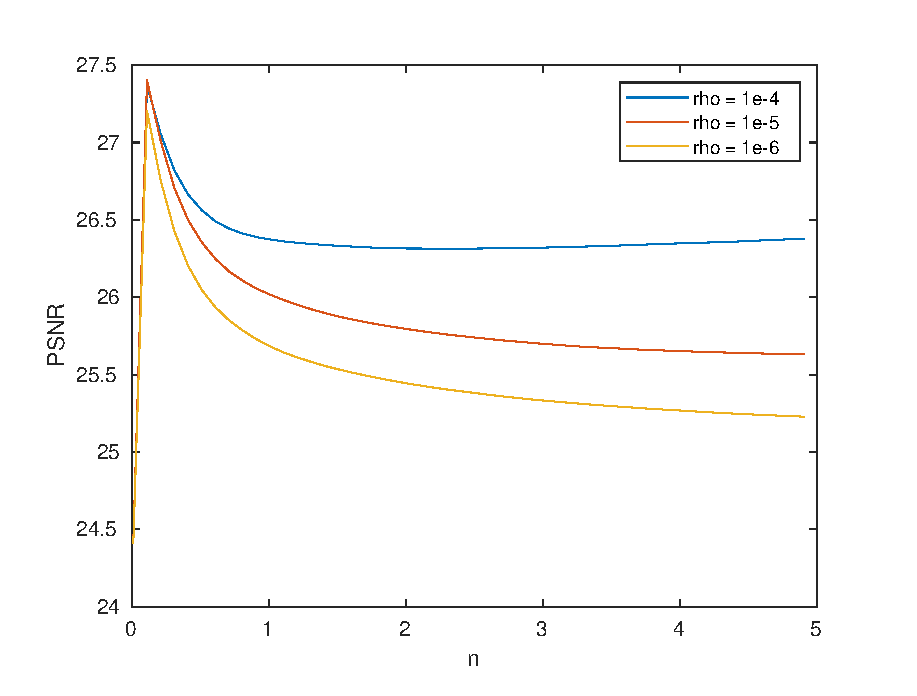
\includegraphics[scale=0.5]{times_beta_serie_psnr.eps}}
        \end{minipage}
       \begin{minipage}[t]{.5\textwidth}
          \centerline{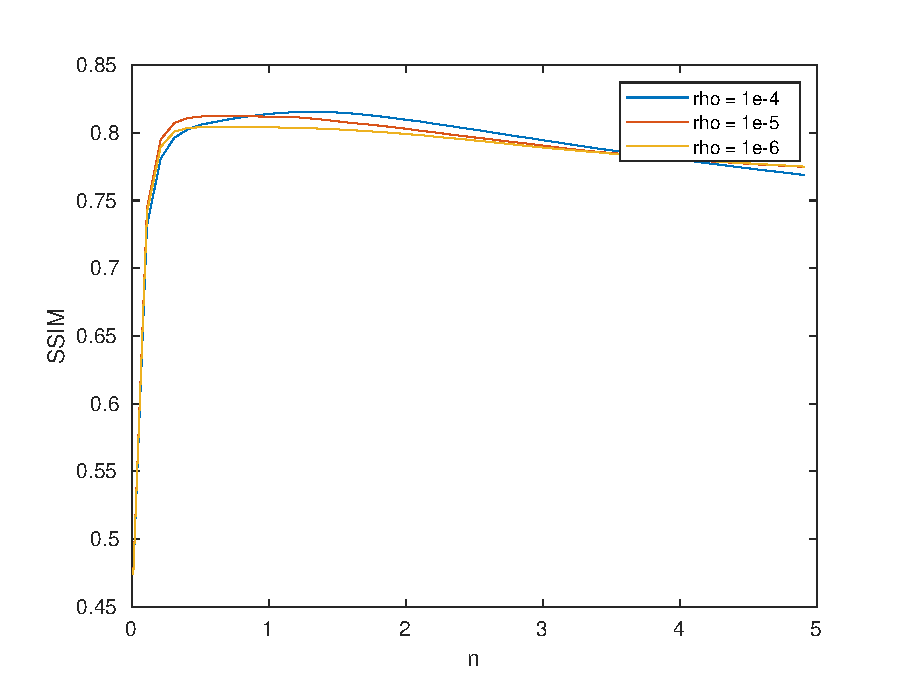
\includegraphics[scale=0.5]{times_beta_serie_ssim.eps}}
        \end{minipage}
        \caption{Variations of PSNR (left) and SSIM (right) with $n= [0.01,5]$}
        \label{fig:test1}
    \end{figure}
    \begin{figure}[h]
        \begin{minipage}[t]{.5\textwidth}
          \centerline{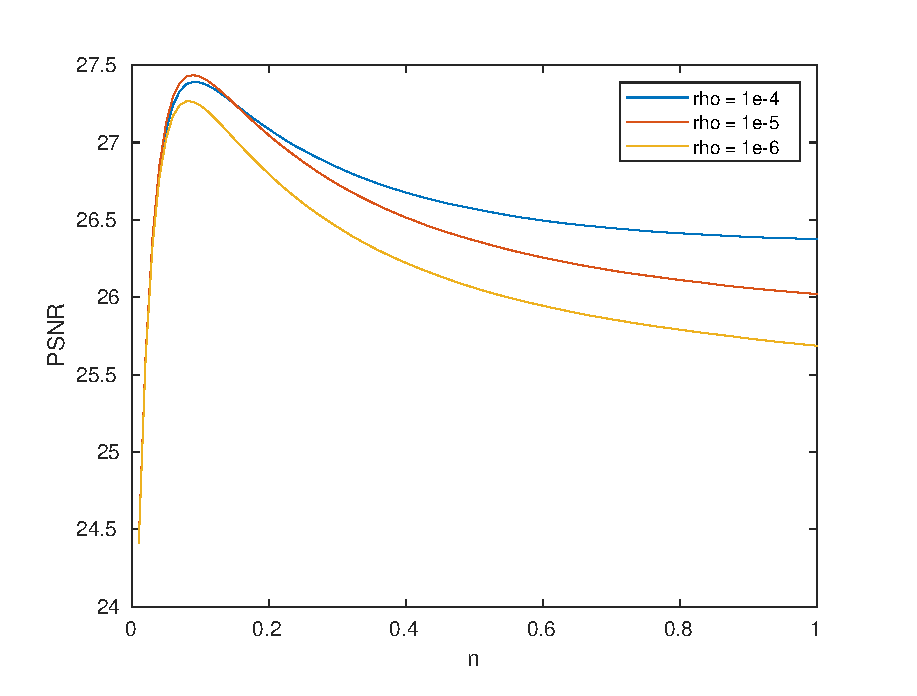
\includegraphics[scale=0.5]{times_serie_psnr2.eps}}
        \end{minipage}
       \begin{minipage}[t]{.5\textwidth}
          \centerline{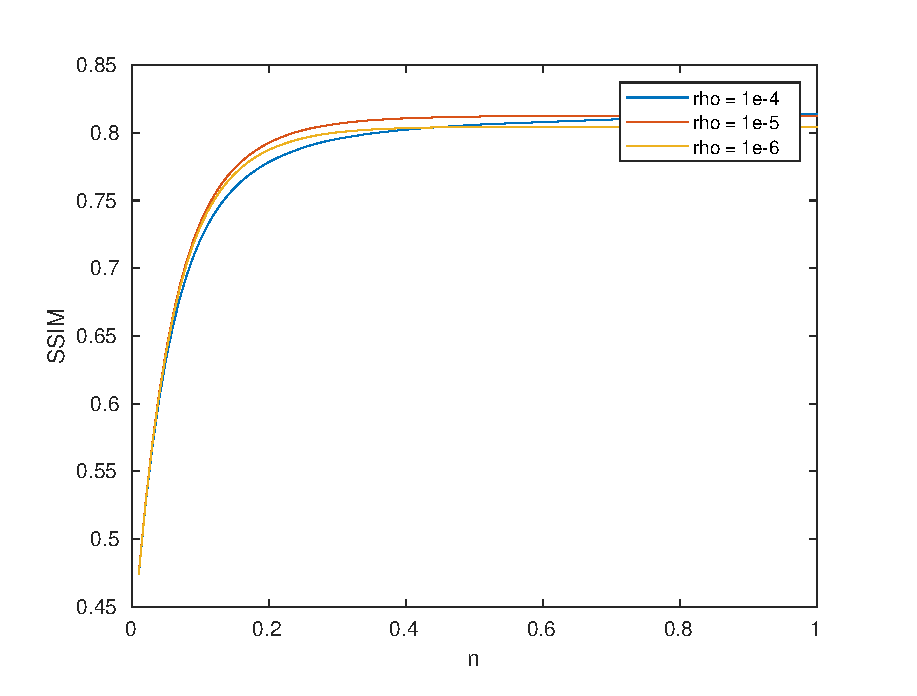
\includegraphics[scale=0.5]{times_serie_ssim2.eps}}
        \end{minipage}
        \caption{Variations of PSNR (left) and SSIM (right) with $n = [0.01,1]$}
        \label{fig:test1 zoom in}
    \end{figure}
    \item For the second test, we apply EPLL for 5 iterations and for each iteration we fix the same $\beta$. We test different $\beta$ on setting $\beta' = \frac{n}{\rho^2}, n = \{0.01,...,30\}$. The PSNR and SSIM curve are shown in Fig. \ref{fig: test2}.
    \begin{figure}[h]
    \begin{minipage}[t]{.5\textwidth}
      \centerline{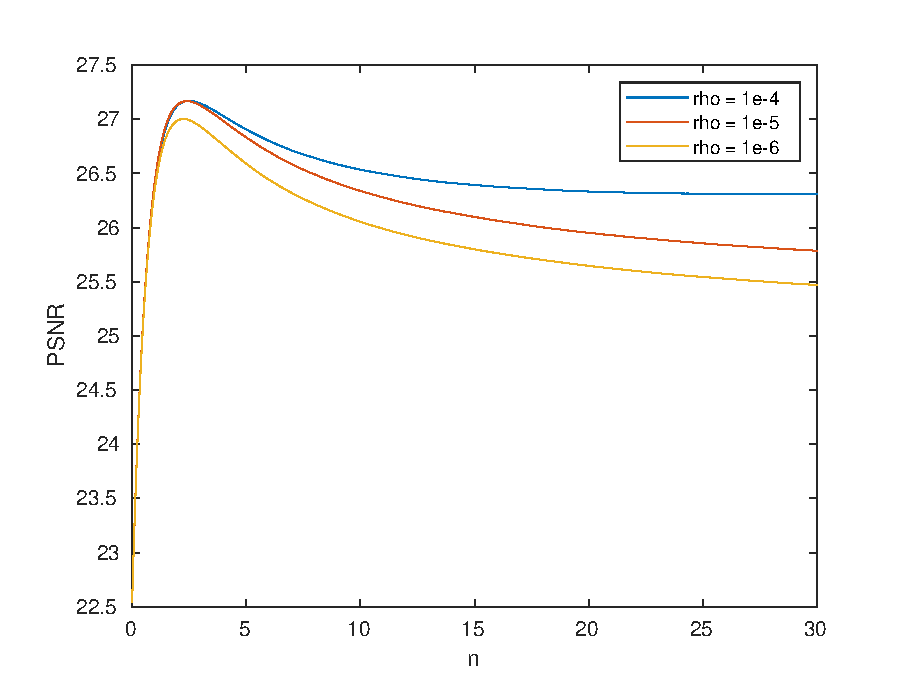
\includegraphics[scale=0.5]{times_beta_psnr.eps}}
    \end{minipage}
   \begin{minipage}[t]{.5\textwidth}
      \centerline{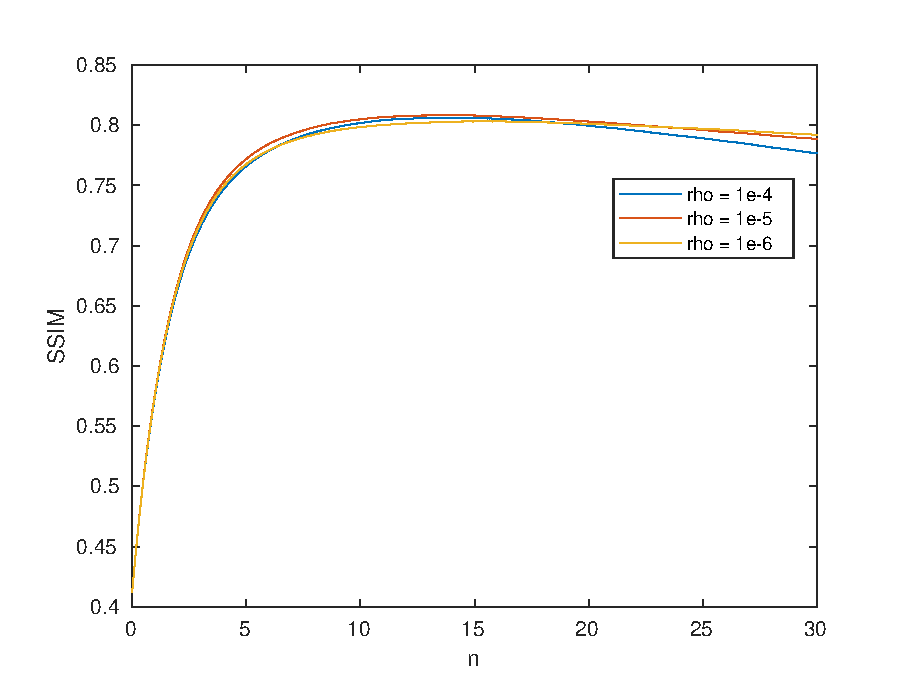
\includegraphics[scale=0.5]{times_beta_ssim.eps}}
    \end{minipage}
    \caption{Variations of PSNR (left) and SSIM (right) with $n = [0.01,30]$}
    \label{fig: test2}
\end{figure}
\end{enumerate}
Based on the Fig. \ref{fig:test1 zoom in} and Fig. \ref{fig: test2}, we find a better $\beta$ for a higher PSNR value with $n = 0.09$ in the first test.
As a summary of these experiments, we simply recommend to use the successive values $\beta =\frac{0.09}{\rho^2}\{1,4,8,16,32\}$ for the 5 iterations of EPLL for optimum results.
We evaluate it with the 3 models for Fig. \ref{fig:diff rho} and obtain results shown in Fig. \ref{fig: beta opt}.
We observe that the average increase of PSNR is 1.23dB with an average drop of SSIM less than 1dB, and we have a better denoising when $\rho^2 = 1e-5$ with the optimal $\beta$. 
\begin{figure}[h]
    \centering
    \begin{tabular}{ccc}
    \rotatebox{90}{$\rho^2=1e-4$} & \includegraphics<\put (0,0){\fcolorbox{white}{white}{\textcolor{black}{27.4/.709}}}>{rho_op_1e-4.eps} & \includegraphics[scale=0.5]<\put (0,0){\fcolorbox{white}{white}{\textcolor{black}{26.5/.720}}}>{rho_op_bar_1e-4.eps}\\
    \rotatebox{90}{$\rho^2=1e-5$} & \includegraphics<\put (0,0){\fcolorbox{white}{white}{\textcolor{black}{27.4/.721}}}>{rho_op_1e-5.eps} & \includegraphics[scale=0.5]<\put (0,0){\fcolorbox{white}{white}{\textcolor{black}{26.4/.725}}}>{rho_op_bar_1e-5.eps}\\
    \rotatebox{90}{$\rho^2=1e-6$} & \includegraphics<\put (0,0){\fcolorbox{white}{white}{\textcolor{black}{27.3/.718}}}>{rho_op_1e-6.eps} & \includegraphics[scale=0.5]<\put (0,0){\fcolorbox{white}{white}{\textcolor{black}{26.5/.724}}}>{rho_op_bar_1e-6.eps}
    \end{tabular}
    \caption{Denoised results using different $\rho^2$ and the optimal $\beta$ with PSNR/SSIM}
    \label{fig: beta opt}
\end{figure}
\subsubsection{Experiments on $K$}
In this Section we focus on the influence of the number of mixture components $K$ for the denoising performance.
The number of $K$ is limited in local patches, we try to find the effect of $K$.
Fig. \ref{fig: k} shows the resulting denoise, restored with EPLL for $K = 5, 20$ and 40.
In this experiments, we use $\rho^2=1e-5$ and $m = 5K(P+P\times r +1)$.
As for the experiments on $\rho ^2$, we have searched the optimal $\beta$ for the models (Fig. \ref{fig:op beta for k}) while applying EPLL within a given range of successive $\beta$ values.
Fig. \ref{fig: k op} shows results with the optimal $\beta$ for PSNR.
Our experiments on $K$ have shown that for our models, there is a significant average gain in PSNR and SSIM when $K$ grows from 0 to 5, that is to say, even with a small $K$, the denoising is functional.
When $K$ increases, the gain increase gets less significant.
Since the computing time is almost linear with $K$, we select $K = 50$ for all the future experiments for a compromise between performance and complexity.
\begin{figure}[h]
    \centering
    \begin{tabular}{ccc}
    \rotatebox{90}{$K=5$} & \includegraphics<\put (0,0){\fcolorbox{white}{white}{\textcolor{black}{26.1/.814}}}>{k_5.eps} & \includegraphics[scale=0.5]<\put (0,0){\fcolorbox{white}{white}{\textcolor{black}{25.1/.745}}}>{k_5_bar.eps}\\
    \rotatebox{90}{$K=20$} & \includegraphics<\put (0,0){\fcolorbox{white}{white}{\textcolor{black}{26.3/.817}}}>{k_20.eps} & \includegraphics[scale=0.5]<\put (0,0){\fcolorbox{white}{white}{\textcolor{black}{25.3/.753}}}>{k_20_bar.eps}\\
    \rotatebox{90}{$K=40$} & \includegraphics<\put (0,0){\fcolorbox{white}{white}{\textcolor{black}{26.6/.823}}}>{k_40.eps} & \includegraphics[scale=0.5]<\put (0,0){\fcolorbox{white}{white}{\textcolor{black}{25.4/.757}}}>{k_40_bar.eps}
    \end{tabular}
    \caption{Denoised results using different $K$ with PSNR/SSIM}
    \label{fig: k}
\end{figure}
\begin{figure}[h]
    \begin{minipage}[t]{.5\textwidth}
      \centerline{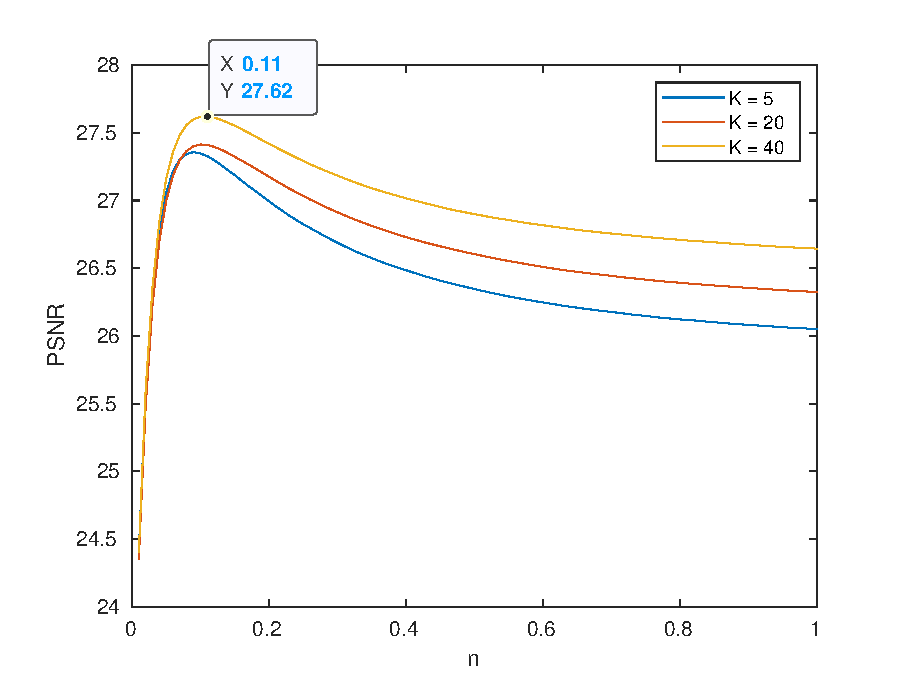
\includegraphics[scale=0.5]{times_beta_k_psnr.eps}}
    \end{minipage}
   \begin{minipage}[t]{.5\textwidth}
      \centerline{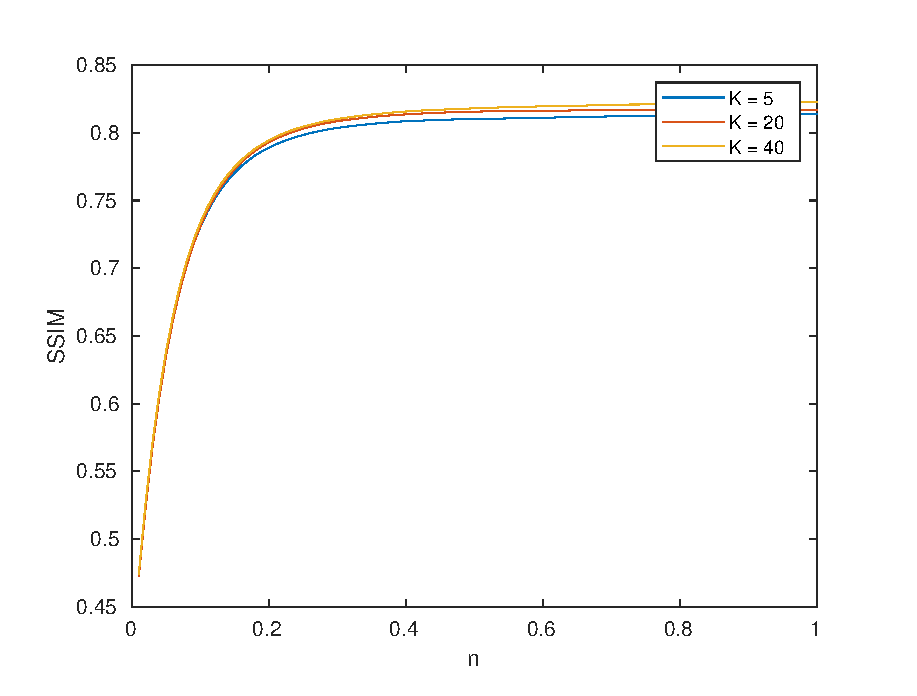
\includegraphics[scale=0.5]{times_beta_k_ssim.eps}}
    \end{minipage}
    \caption{Variations of PSNR (left) and SSIM (right) with $n = [0.01,1]$}
    \label{fig:op beta for k}
\end{figure}
\begin{figure}[h]
    \centering
    \begin{tabular}{ccc}
    \rotatebox{90}{$K=5$} & \includegraphics<\put (0,0){\fcolorbox{white}{white}{\textcolor{black}{27.3/.741}}}>{k5_op.eps} & \includegraphics[scale=0.5]<\put (0,0){\fcolorbox{white}{white}{\textcolor{black}{26.3/.736}}}>{k5_op_bar.eps}\\
    \rotatebox{90}{$K=20$} & \includegraphics<\put (0,0){\fcolorbox{white}{white}{\textcolor{black}{27.4/.743}}}>{k20_op.eps} & \includegraphics[scale=0.5]<\put (0,0){\fcolorbox{white}{white}{\textcolor{black}{26.5/.740}}}>{k20_op_bar.eps}\\
    \rotatebox{90}{$K=40$} & \includegraphics<\put (0,0){\fcolorbox{white}{white}{\textcolor{black}{27.6/.745}}}>{k40_op.eps} & \includegraphics[scale=0.5]<\put (0,0){\fcolorbox{white}{white}{\textcolor{black}{26.6/.741}}}>{k40_op_bar.eps}
    \end{tabular}
    \caption{Denoised results using different $K$ and optimal $\beta$ for PSNR}
    \label{fig: k op}
\end{figure}
\subsubsection{Experiments on $m$}
From \cite{keriven:hal-01329195} we know that the performance of model reconstruction is proportional to the number of free parameters $K(P + P\times r + 1)$ in diagonal GMMs.
To find the minimal size of sketch for our model, we evaluate the denoising quality with respect to the number of frequencies $m$ by setting $m = c\times K(P + P\times r + 1)$.
For the below experiences, we compress $2 \times 10^6$ patches extract from the database BSDS as in \cite{deledalle:hal-01700082} and learn the models for $K = 50$.
Compromising the denoising performance and the computing time, we set the number of iterations during sketching $itr = 5$ instead of 100 for the following experiments.
From top to bottom Fig. \ref{fig: c op} shows the results of $c = 1, 2$ and 5 with optimal $\beta$ values.
Comparing with the results restored with EPLL with EM prior (Fig. \ref{fig: em}) learned from 2 millions of patches at $K = 50$, our models don't show satisfy results as expected.
Therefore, we do more experiments and observe the models' energy by setting $ m = 2K(P + P\times r + 1$, augmenting the number of iterations.
\begin{figure}[h]
    \centering
    \begin{tabular}{ccc}
    \rotatebox{90}{$c=1$} & \includegraphics<\put (0,0){\fcolorbox{white}{white}{\textcolor{black}{27.2/.722}}}>{c1_it5_ca.eps} &\includegraphics[scale=0.5]<\put (0,0){\fcolorbox{white}{white}{\textcolor{black}{26.4/.726}}}>{c1_it5_bar.eps}\\
    \rotatebox{90}{$c=2$} & \includegraphics<\put (0,0){\fcolorbox{white}{white}{\textcolor{black}{27.4/.732}}}>{c2_it5_ca.eps} & \includegraphics[scale=0.5]<\put (0,0){\fcolorbox{white}{white}{\textcolor{black}{26.5/.733}}}>{c2_it5_bar.eps}\\
    \rotatebox{90}{$c=5$} & \includegraphics<\put (0,0){\fcolorbox{white}{white}{\textcolor{black}{27.4/.723}}}>{c5_it5_ca.eps} & \includegraphics[scale=0.5]<\put (0,0){\fcolorbox{white}{white}{\textcolor{black}{26.5/.728}}}>{c5_it5_bar.eps}
    \end{tabular}
    \caption{Denoised results with different $m$ (optimal $\beta$ for PSNR)}
    \label{fig: c op}
\end{figure}
\begin{figure}[h]
\begin{minipage}[t]{.5\textwidth}
\includegraphics[scale=0.38]<\put (0,0){\fcolorbox{white}{white}{\textcolor{black}{29.9/.868}}}>{em_0.eps}
\end{minipage}
   \begin{minipage}[t]{.5\textwidth}
\includegraphics[scale=0.5]<\put (0,0){\fcolorbox{white}{white}{\textcolor{black}{29.4/.864}}}>{em_k50_0_bar.eps}
\end{minipage}
\caption{Denoised results with EM}
\label{fig: em}
\end{figure}
\subsubsection{Other experiments}
We vary the iteration numbers during the sketching by setting $itr = 5$, 20 and 50, denoising results are shown in Fig. \ref{fig: itr} with optimal $\beta$.
To one's surprise, models with more iteration numbers during the learning process have worse denoising performance.
In Fig. \ref{fig: energy} and \ref{fig: energy_c5k20} we can see that those models' energy decrease and hit a plateau faster.
We also compare the models' energy of different number of iterations during sketch learning with the model learned by EM, the results are shown in Table \ref{tab:energy-table}.
\begin{figure}[h]
\begin{tabular}{cc}
      \includegraphics<\put (0,0){\fcolorbox{white}{white}{\textcolor{black}{itr=10:26.5/.717}}}>{c2_it10.eps} & \includegraphics<\put (0,0){\fcolorbox{white}{white}{\textcolor{black}{itr=20:26.2/.714}}}>{c2_it20.eps}\\
      \includegraphics<\put (0,0){\fcolorbox{white}{white}{\textcolor{black}{itr=50:26.1/.705}}}>{c2_it50.eps} & \includegraphics<\put (0,0){\fcolorbox{white}{white}{\textcolor{black}{itr=100:26.5/.715}}}>{c2_it100.eps}
\end{tabular}
    \caption{Denoised results with different number of iterations(optimal $\beta$ for PSNR)}
    \label{fig: itr}
\end{figure}

\begin{table}[h]
\begin{tabular}{|c|c|c|c|c|c|}
\hline
EM     &itr = 100 &itr = 50    & itr = 20   & itr = 10  & itr = 5 \\ \hline
1.6971e+03 & 819.7625 & 1.9218e+3 & 1.9226e+03 & 2.1068e+03 & 2.2764e+03 \\ \hline

% \multicolumn{1}{|c|}{c =5,k20} &2.0245e+03 &  &  &  &1.3574e+03 & 3.2654e+03(3.1819e+03 for $\rho^2 = 1e-4)$ \\ \hline
\end{tabular}
\caption{Table of model energy compute with sketch c = 2, k= 5}
\label{tab:energy-table}
\end{table}
\begin{figure}[h]
\includegraphics[scale=1]<\put (62,1.5){\fcolorbox{white}{white}{\textcolor{black}{$T$}}}>{energy_curve_it.eps}
\caption{Log energy curve for model at $c=2,K =50$}
\label{fig: energy}
\end{figure}
\begin{figure}[h]
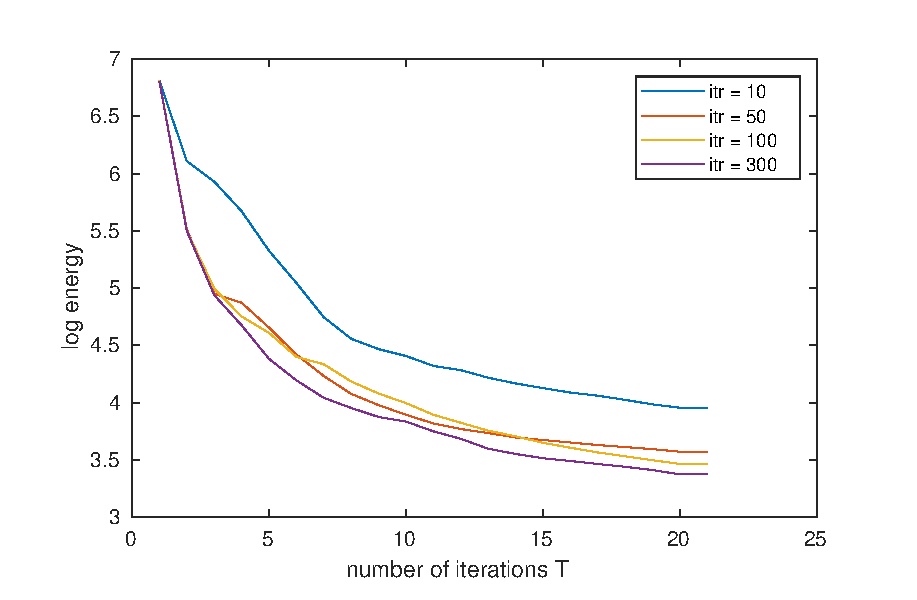
\includegraphics[scale=1]{energy_c5k20.eps}
\caption{Log energy curve for model at $c=5,K =20$}
\label{fig: energy_c5k20}
\end{figure}


\section{Conclusion}
In this work, we provide a implementation of sketching model and we show how the parameters of models influence the denoising performance.
It is shown that a probabilistic high-dimensional Gaussian mixture model can be learned from a compression of a big database of patches, and used to patch-based denoising. 
However, the resulting models of sketching have not achieved state of the art denoising performances, the proposed method isn't practical enough in terms of computing complexity.
This work opens several perspectives. 
The first one concerns the possibility to impose an hyperprior on the GMM parameters to stabilize the estimation procedure, as was shown in \cite{houdard:hal-01544249}.
The actual model we implement use the principle of MPPCA \cite{mppca} (the mixture of probabilistic principal component analyzers), assumes that the data have a common intrinsic dimensionality and that the noise is an isotropic noise: the rank $r_k$ are the same for all groups $k$ and we decompose $\Sigma_k$ with $svds(\Sigma_k, r)$.
However, the authors of \cite{wang2013sure} noticed that the fact that all groups must have the same intrinsic dimension in MPPCA is a limit for image denoising as in \cite{parameswaran:hal-01617722} and \cite{wang2013sure}.
Therefore, we propose to add a step to estimate $r_k$ for each group $k$ before decompose $\Sigma_k$ using Algo. \ref{algo:3} proposed in \cite{houdard:hal-01544249} for a finer modeling. 
Another possible direction is the application of the estimation algorithm proposed in \cite{traonmilin:hal-01938239} in order to overcome the limitation encountered in the actual algorithm. 
Another possible extension would be the generalization of the sketching model to more general restoration problem once it realize state of the art denoising performances.
\begin{algorithm}[H]
 \KwData{$K$ sets of the eigenvalues $\lambda_{k1},...,\lambda_{kp}$ for each gaussian }
 \KwResult{The dimensions $r_k$ for each $k$}
 
 \For{k = 1 \textbf{to} $K$ }{
 $r_k \xleftarrow{} \argmin \left\| mean(\lambda_{kr+1},...,\lambda_{kP})-\rho\right\|$\\
 $(r_k \xleftarrow{} \argmin_r \left\|\frac{1}{P-r} \sum_{j = r+1}^P \lambda_{kj}-\rho^2\right\|)$ where $\lambda_{kj}$ the j-th largest eigenvalue of the empirical covariance matrix of component k
 }
 \caption{Intrinsic dimension estimation for a given value of $\rho^2$}
 \label{algo:3}
\end{algorithm}
\newpage
\bibliographystyle{plain}
\bibliography{refs}



\end{document}